\documentclass[preprint,12pt,authoryear=false]{elsarticle}

\usepackage[utf8]{inputenc}
\usepackage[T1]{fontenc}
\usepackage[brazil]{babel}
\usepackage{lmodern}
\usepackage[a4paper,top=22mm,bottom=24mm,left=28mm,right=28mm]{geometry}
\usepackage{amsmath,amssymb}
\usepackage{graphicx}
\usepackage{booktabs}
\usepackage{longtable}
\usepackage{tabularx}
\usepackage{multirow}
\usepackage{xcolor}
\usepackage{tikz}
\usetikzlibrary{positioning,arrows.meta,calc}
\usepackage[hidelinks]{hyperref}
\usepackage{lineno}
\linenumbers

% ---------------------------------------------------------------
% Notas dos autores. Cada \pendente{} marca trabalho que ainda
% depende de dados novos ou de uma decisão dos autores. Remover
% todos antes da submissão (buscar por "PENDENTE").
% ---------------------------------------------------------------
\newcommand{\pendente}[1]{\textcolor{red}{\textbf{[PENDENTE:} #1\textbf{]}}}

\newcommand{\PM}{TF-PM}
\newcommand{\ST}{TF-ST}
\newcommand{\FC}{TF-FC}
\newcommand{\MSR}{TF-MSR}

\abstracttitle{Resumo}
\keywordtitle{Palavras-chave}
\makeatletter
\def\@elsarticlehighlightstitle{Destaques}
\def\ps@pprintTitle{\let\@oddhead\@empty\let\@evenhead\@empty\def\@oddfoot{\hfill\thepage\hfill}\let\@evenfoot\@oddfoot}
\makeatother
\renewcommand{\appendixname}{Apêndice}

\journal{Information and Software Technology}

\begin{document}

\begin{frontmatter}

\title{Mineração de Processos, Modelagem Estocástica e Previsão de Processos de Desenvolvimento de Software: Um Estudo de Mapeamento Sistemático}

\author[pucpr]{Rodrigo Almeida de Oliveira\corref{cor1}}
\ead{rodrigo.almeida1@pucpr.edu.br}
\author[pucpr]{Juliano de Paulo Ribeiro}
\ead{juliano.ribeiro@pucpr.edu.br}
\author[pucpr]{Edson Emilio Scalabrin}
\ead{scalabrin@ppgia.pucpr.br}
\cortext[cor1]{Autor correspondente.}
\affiliation[pucpr]{organization={Pontifícia Universidade Católica do Paraná (PUCPR), Programa de Pós-Graduação em Informática (PPGIa)},
  city={Curitiba}, state={PR}, country={Brasil}}

\begin{abstract}\small
\textbf{Contexto.} Repositórios de software registram o desenvolvimento como eventos com carimbo de tempo. A mineração de processos (PM), a modelagem estocástica e a previsão de métricas de processo exploram esses rastros, em grande parte de forma independente.
\textbf{Objetivo.} Mapear os estudos primários que aplicam essas técnicas a dados de desenvolvimento de software, caracterizar como as três linhas evoluíram e medir até que ponto elas foram integradas.
\textbf{Método.} Um estudo de mapeamento sistemático relatado segundo o SEGRESS. Cinco bibliotecas digitais e uma iteração de busca por citações resultaram em 5.783 registros únicos (12 de abril de 2026). Um modelo de linguagem serviu de apoio a uma primeira triagem; todo registro que ele excluiu ou deixou sem decisão foi triado novamente por dois revisores humanos. Os estudos foram classificados em quatro famílias de técnica e de dados e em quatro níveis de integração (L0--L3).
\textbf{Resultados.} O corpus contém 456 estudos publicados entre 1994 e 2026, dos quais 380 estão classificados. A modelagem estocástica (55,3\%) predominou até 2013; a mineração de processos (41,3\%) predomina desde 2014. As duas linhas se encontram em 10 estudos. A previsão aparece em 29,2\% dos estudos, quase sempre associada a modelos estocásticos (90 estudos) e raramente à mineração de processos (7). Um estudo combina as três famílias (L2), e nenhum as acopla por meio de interfaces especificadas e avaliadas de ponta a ponta (L3).
\textbf{Conclusão.} A área está fragmentada segundo as comunidades de pesquisa, e não por falta de técnicas. A previsão estocástica orientada a processos, na qual a estrutura de processo minerada parametriza uma previsão estocástica, é a combinação menos explorada. Propõe-se uma agenda com quatro direções.
\end{abstract}

\begin{highlights}
\item 456 estudos aplicam PM, modelos estocásticos ou previsão a dados do SDLC.
\item A modelagem estocástica predominou até 2013; desde então, a mineração de processos.
\item PM e modelagem estocástica se encontram em 10 dos 380 estudos classificados.
\item Um estudo combina as três; nenhum as acopla com avaliação de ponta a ponta.
\item Corpus, classificação e registros de triagem estão disponíveis abertamente.
\end{highlights}

\begin{keyword}
Estudo de mapeamento sistemático \sep Mineração de processos \sep Modelagem estocástica \sep Previsão de processos de software \sep Mineração de repositórios de software
\end{keyword}

\end{frontmatter}

% =================================================================
\section{Introdução}\label{sec:intro}

Organizações de software precisam responder rotineiramente a perguntas de previsão sobre o próprio processo de desenvolvimento: quando uma funcionalidade será entregue, quanto tempo uma issue permanecerá aberta ou se uma release vai atrasar. Os dados necessários para respondê-las já existem como subproduto do trabalho cotidiano. Commits, transições de issues, pull requests, revisões de código e execuções de CI/CD são todos eventos com carimbo de tempo.

Três comunidades de pesquisa desenvolveram técnicas capazes de explorar esses rastros, em grande parte de forma independente umas das outras. A mineração de processos (PM, do inglês \emph{process mining}) descobre, verifica e aprimora modelos de processo a partir de logs de eventos, e é aplicada a repositórios de software desde os trabalhos de Cook e Wolf~\cite{cook1995,cook1998} e de Rubin et al.~\cite{rubin2007}. A modelagem estocástica, incluindo cadeias de Markov, redes de Petri estocásticas e simulação de Monte Carlo, tem longa tradição em confiabilidade de software e em simulação de processos~\cite{whittaker1994,ali2014}. A predição baseada em aprendizado de máquina domina a pesquisa em mineração de repositórios de software sobre defeitos, esforço e resultados~\cite{kagdi2007,hall2012} e, na gestão de processos de negócio, o monitoramento preditivo de processos~\cite{marquez2018}.

Combinar as três é atraente porque cada uma cobre uma fraqueza das outras. A PM fornece uma estrutura de processo fundamentada empiricamente. Os modelos estocásticos transformam essa estrutura em distribuições de probabilidade sobre caminhos e durações futuros. Os modelos aprendidos podem corrigir erros sistemáticos usando atributos de contexto. Não se sabe se essas combinações já foram construídas, nem sobre quais dados.

\paragraph{Estudos secundários relacionados}
Os estudos secundários existentes cobrem, cada um, um lado desse espaço. O monitoramento preditivo de processos foi revisado e comparado em \emph{benchmarks} para predição de resultado~\cite{teinemaa2019}, predição de tempo restante~\cite{verenich2019}, métodos de aprendizado profundo~\cite{ramamaneiro2023} e de modo geral~\cite{marquez2018}, mas sobre logs de eventos de negócio, e não sobre processos de desenvolvimento de software. Os mapeamentos gerais de aplicações de mineração de processos~\cite{garcia2019,thiede2018} tratam a engenharia de software como um domínio entre muitos e não abordam previsão. Dentro da engenharia de software, estudos secundários cobriram a modelagem por simulação de processos~\cite{zhang2010,ali2014}, a mineração de processos em logs de eventos de software livre (FLOSS)~\cite{mukala2015}, a mineração de processos de software com redes de Petri~\cite{thamizharasan2016}, o monitoramento contínuo de software apoiado por mineração de processos~\cite{stepanov2026}, a mineração de repositórios~\cite{kagdi2007} e a predição de defeitos~\cite{hall2012}. Nenhum mapeia o uso conjunto de mineração de processos, modelagem estocástica e previsão sobre dados de desenvolvimento de software.

\paragraph{Contribuições}
Este artigo relata um estudo de mapeamento sistemático dessa interseção. Suas contribuições são:
\begin{enumerate}
\item um corpus de 456 estudos primários, disponível abertamente junto com os registros de triagem e de classificação;
\item uma classificação dos estudos em quatro famílias de técnica e de dados e em quatro níveis de integração, com a evolução de cada família ao longo de três décadas; e
\item uma análise das lacunas entre as três linhas de pesquisa, da qual derivamos uma agenda de pesquisa com quatro direções.
\end{enumerate}

A revisão foi motivada pelo trabalho dos próprios autores em um pipeline integrado de previsão. Relatamos isso porque é uma possível fonte de viés na forma como os níveis de integração foram definidos e interpretados; por isso, as definições da Seção~\ref{sec:classification} são enunciadas sem referência a nenhuma arquitetura específica, e a ameaça é discutida na Seção~\ref{sec:threats}.

A Seção~\ref{sec:method} descreve o protocolo da revisão; a Seção~\ref{sec:selection}, os resultados da busca e da seleção; a Seção~\ref{sec:results}, as respostas às questões de pesquisa; a Seção~\ref{sec:discussion}, a discussão e a agenda de pesquisa; a Seção~\ref{sec:threats}, as ameaças à validade; e a Seção~\ref{sec:conclusion} conclui.

% =================================================================
\section{Protocolo da Revisão}\label{sec:method}

Seguimos as diretrizes de mapeamento de Petersen et al.~\cite{petersen2015}, as diretrizes de Kitchenham e Charters~\cite{kitchenham2007} e o procedimento de \emph{snowballing} de Wohlin~\cite{wohlin2014}, e relatamos segundo o SEGRESS~\cite{segress}. O protocolo do mapeamento não foi registrado previamente. O checklist SEGRESS preenchido está no material suplementar.

\subsection{Questões de pesquisa}\label{sec:rqs}

\begin{description}
\item[RQ1] Como evoluiu a pesquisa que aplica mineração de processos, modelagem estocástica ou previsão a dados de desenvolvimento de software?
\item[RQ2] Quais famílias de técnica, e quais combinações entre elas, os estudos utilizam?
\item[RQ3] Quais fases do SDLC, fontes de logs de eventos e técnicas específicas os estudos abordam?
\item[RQ4] Em que medida a mineração de processos, a modelagem estocástica e a previsão estão integradas, e quais lacunas permanecem?
\end{description}

RQ1 e RQ2 caracterizam o corpus. RQ3 descreve o que os estudos analisam e com quais algoritmos. RQ4 trata da questão que motivou esta revisão.

\pendente{RQ3 só pode ser respondida após a extração humana dos campos fase do SDLC, fonte e construção do event log, algoritmo de PM, método estocástico e alvo da previsão (ver Seção~\ref{sec:rq3}). A extração anterior, feita pelo LLM, teve 0\% de concordância exata com o avaliador humano e não pode ser usada. Se a extração não for feita, retirar RQ3 do artigo.}

\subsection{Estratégia de busca}\label{sec:search}

A busca automatizada cobriu cinco bibliotecas digitais: IEEE Xplore, ACM Digital Library, Scopus, Web of Science e SpringerLink. As strings foram construídas a partir de uma decomposição PICO adaptada à engenharia de software. A população é o contexto de engenharia de software (desenvolvimento de software, SDLC, DevOps, CI/CD, rastreamento de issues, controle de versão, revisão de código). A intervenção é a técnica analítica (mineração de processos, descoberta de processos, verificação de conformidade, monitoramento preditivo de processos, cadeia de Markov, Monte Carlo, rede de Petri estocástica). O resultado é uma previsão ou um modelo de processo (\emph{lead time}, tempo de ciclo, tempo restante, vazão). Não há faceta de comparação.

Foram derivadas três listas de termos complementares: uma string principal que une população e intervenção; uma string complementar para estudos que usam a terminologia de MSR sem os termos canônicos de PM; e uma string de fronteira para a interseção entre métodos estocásticos e PM em contextos de software. Elas foram adaptadas a cada biblioteca, resultando em 25 exportações (Tabela~\ref{tab:search}). Todas as buscas foram executadas em 12 de abril de 2026, com janela de publicação de 1º de janeiro de 1994 (Whittaker e Thomason~\cite{whittaker1994}) até essa data. As publicações datadas de 2026 representam, portanto, cobertura parcial do ano. As listas de termos compartilhadas estão no \ref{app:strings}; todas as strings específicas de cada base estão no pacote de replicação.

\pendente{Três strings do Scopus contêm os títulos literais de artigos do conjunto de controle (V6, V8, V9). Opção A: retirar os títulos, rodar as strings de novo e atualizar as Tabelas~\ref{tab:search} e~\ref{tab:selection}. Opção B: manter, deixando a declaração da Seção~\ref{sec:threats-search}, e validar a busca com um conjunto de teste independente.}

\pendente{Nenhuma string principal tem bloco de forecasting/ML em repositórios (por exemplo ``bug fix time'', ``issue resolution time'', ``effort estimation'', ``machine learning'')~\cite{panjer2007,giger2010}. Rodar esse bloco nas cinco bases e incorporar os resultados ao corpus. A busca suplementar no Scopus de 31/10/2026 (165 registros, 19 includes por título) deve ser incorporada ou descartada de vez.}

\begin{table}[t]
\centering\small
\caption{Registro das buscas por fonte. Todas as exportações foram obtidas em 12 de abril de 2026. Os registros únicos são contados uma vez, na fonte que forneceu a cópia mantida.}\label{tab:search}
\footnotesize
\begin{tabular}{lllrr}
\toprule
Fonte & Campo & Exportações & Brutos & Únicos \\
\midrule
Scopus & TITLE-ABS-KEY & 6 & 2.377 & 1.852 \\
SpringerLink & Busca simplificada & 10 & 2.884 & 1.543 \\
IEEE Xplore & Todos os metadados & 17 lotes & 1.386 & 1.263 \\
Web of Science & Tópico (TS) & 4 & 997 & 514 \\
ACM DL & Resumo & 2 + 1 exportação & 96 & 34 \\
\emph{Snowballing} & -- & 1 iteração & 595 & 575 \\
Conjunto de controle & -- & -- & 12 & 2 \\
\midrule
Total & & & 8.347 & 5.783 \\
\bottomrule
\end{tabular}
\end{table}

\paragraph{\emph{Snowballing}}
Uma iteração de \emph{snowballing} para trás e para a frente foi executada sobre 400 DOIs de origem e recuperou 595 registros. Um candidato era mantido quando seu título ou resumo continha um termo de PM ou estocástico e um termo de engenharia de software.

\pendente{O procedimento acima não segue Wohlin~\cite{wohlin2014}: os 400 DOIs-fonte não são os estudos incluídos, backward e forward não estão separados e não houve critério de saturação. Refazer o snowballing a partir dos 380 estudos classificados, separando backward e forward e iterando até nenhum estudo novo aparecer, e informar as contagens por iteração. Sem isso, descrever o procedimento como ``uma iteração de busca por citações'' e não como snowballing de Wohlin.}

\paragraph{Conjunto de controle}
Dez estudos conhecidos (Tabela~\ref{tab:control}) foram usados para verificar se as strings recuperam trabalhos relevantes. Todos os dez foram recuperados. Como os dez já eram conhecidos quando as strings foram escritas, essa verificação não estima a sensibilidade da busca.

\begin{table}[t]
\centering\small
\caption{Estudos de controle para a verificação das strings de busca.}\label{tab:control}
\footnotesize
\begin{tabularx}{\textwidth}{llXl}
\toprule
\# & Estudo & Justificativa & Recuperado via \\
\midrule
V1 & Cook \& Wolf (1998) & PM seminal em ES & ACM \\
V2 & Rubin et al. (2007) & Framework de PM para processos de software & Scopus \\
V3 & Poncin et al. (2011) & PM e MSR & IEEE \\
V4 & Caldeira \& Cardoso (2019) & PM para avaliação de processos de software & IEEE \\
V5 & Lemos et al. (2011) & PM para gestão de processos de software & IEEE \\
V6 & Whittaker \& Thomason (1994) & Modelos de Markov em teste de software & Scopus \\
V7 & Tax et al. (2017) & Monitoramento preditivo de processos (BPM) & Conjunto de controle \\
V8 & Rogge-Solti \& Weske (2015) & Previsão com PM estocástica & Scopus \\
V9 & Rozinat et al. (2009) & Da PM à simulação & Conjunto de controle \\
V10 & Gupta \& Sureka (2017) & PM em múltiplos repositórios em ES & ACM \\
\bottomrule
\end{tabularx}
\end{table}

\subsection{Critérios de elegibilidade}\label{sec:criteria}

A Tabela~\ref{tab:criteria} lista os critérios. A unidade de contagem é a publicação~\cite{petersen2015}. Registros duplicados da mesma publicação são unificados. Um artigo de conferência e sua extensão posterior são ambos mantidos quando cada um satisfaz os critérios de forma independente; há dois desses pares no corpus, e contá-los uma única vez não alteraria nenhum percentual relatado em mais de um ponto.

Um estudo é incluído quando satisfaz IC1--IC3 e ao menos um dos critérios de conteúdo IC4a--IC4d, e nenhum de EC1--EC5. Os quatro critérios de conteúdo definem as quatro famílias usadas ao longo do artigo: \PM{} (IC4a), \ST{} (IC4b), \FC{} (IC4c) e \MSR{} (IC4d). \PM{}, \ST{} e \FC{} são famílias de técnica; \MSR{} descreve a fonte de dados.

\pendente{IC4b e IC4c, como estão, aceitam modelos Markovianos de teste estatístico e modelos de crescimento de confiabilidade (``defect rates''). Esses modelos descrevem o produto, não o processo de desenvolvimento, e provavelmente formam boa parte dos 89 estudos ST+FC de 1997--2013. Decidir: (a) mantê-los, declarando o escopo amplo; ou (b) acrescentar um EC (``model of product reliability, not of the development process'') e reclassificar.}

\begin{table}[t]
\centering\small
\caption{Critérios de inclusão e exclusão.}\label{tab:criteria}
\begin{tabularx}{\textwidth}{llX}
\toprule
Tipo & ID & Critério \\
\midrule
\multirow{7}{*}{Inclusão}
 & IC1 & Publicado entre 1º de janeiro de 1994 e 12 de abril de 2026. \\
 & IC2 & Escrito em inglês. \\
 & IC3 & Artigo de periódico, de conferência ou de workshop revisado por pares, com ao menos quatro páginas. \\
 & IC4a & Aplica mineração de processos (descoberta, verificação de conformidade, monitoramento preditivo de processos) a artefatos de desenvolvimento de software (commits, issues, pull requests, logs de CI/CD, rastreadores de bugs, controle de versão). \\
 & IC4b & Usa modelos estocásticos (cadeias de Markov, Monte Carlo, redes de Petri estocásticas, cadeias absorventes) para analisar processos ou fluxos de trabalho de desenvolvimento de software. \\
 & IC4c & Propõe ou avalia a previsão de métricas de processo de software (\emph{lead time}, tempo de ciclo, tempo restante, vazão, taxas de defeitos) a partir de logs de eventos ou de dados de repositório. \\
 & IC4d & Minera repositórios de software (GitHub, Jira, controle de versão, plataformas de CI/CD) para descobrir, analisar ou melhorar modelos de processo de software. \\
\midrule
\multirow{5}{*}{Exclusão}
 & EC1 & Domínio de aplicação exclusivamente fora do desenvolvimento de software, sem relevância demonstrada para processos do SDLC. \\
 & EC2 & O software é apenas a plataforma de implementação; o processo analisado não é um processo de desenvolvimento de software. \\
 & EC3 & Contribuição puramente algorítmica ou teórica, sem avaliação empírica em contexto de desenvolvimento de software. \\
 & EC4 & Estudo secundário que não trata especificamente de PM ou de métodos estocásticos em engenharia de software. \\
 & EC5 & O registro não pode ser julgado com a evidência obtida: texto completo não recuperável (EC5a), sem resumo e sem texto completo (EC5b) ou informação decisiva ausente (EC5c). \\
\bottomrule
\end{tabularx}
\end{table}

\subsection{Processo de seleção}\label{sec:selection-process}

A seleção teve três etapas.

\paragraph{Etapa 1: primeira triagem apoiada por modelo de linguagem}
Um modelo de linguagem (claude-haiku-4-5-20251001, Message Batches API da Anthropic) triou todos os registros únicos segundo IC4a--IC4d e EC1--EC4, retornando \emph{incluir}, \emph{excluir} ou \emph{talvez}, com uma justificativa curta. Os registros marcados como incluir ou talvez foram encaminhados a uma segunda passagem, mais estrita, sobre título e resumo (\emph{incluir}, \emph{excluir} ou \emph{pendente}). Antes disso, os resumos ausentes nas exportações foram recuperados no Semantic Scholar, OpenAlex, CORE e Crossref. Os prompts, os esquemas JSON e as decisões por registro estão no pacote de replicação.

\paragraph{Etapa 2: verificação humana da primeira triagem}
Dois avaliadores, cegos em relação às decisões do modelo e um ao outro, julgaram uma amostra aleatória estratificada de 177 decisões da segunda passagem segundo a Tabela~\ref{tab:criteria}. A concordância entre avaliadores antes do consenso foi $\kappa = 0{,}654$. Em relação ao consenso, a primeira triagem manteve 29 dos 46 estudos elegíveis amostrados (Recall 0,630; IC de Wilson 95\% 0,486--0,755). Para os registros do segundo lote de triagem, amostras estratificadas das não inclusões do modelo indicaram um Recall estimado de 0,563. O critério de sucesso fixado antes dessa verificação era um Recall de no mínimo 0,90. Como ele não foi atingido, a primeira triagem é usada aqui apenas para priorizar registros, e a Etapa~3 triou novamente todos os registros que ela não incluiu.

\pendente{Informar onde o pré-registro da verificação foi depositado, com carimbo de tempo verificável (OSF ou Zenodo, com DOI ou link).}

\paragraph{Etapa 3: re-triagem humana e verificação das inclusões}
Dois revisores triaram todos os 4.005 registros que a primeira triagem havia excluído ou deixado sem decisão, incluindo 611 registros encerrados sem decisão por falta de resumo. Eles também verificaram cada inclusão da primeira triagem segundo os critérios. A re-triagem identificou 188 registros elegíveis, que, após a remoção de duplicatas e uma verificação final de elegibilidade, acrescentaram 150 estudos. A verificação das inclusões removeu 32 estudos cujo título e resumo não sustentavam a inclusão.

\pendente{Para tornar a Etapa~3 auditável: (a) registrar, por linha, a decisão de cada revisor, separada da sugestão exibida, e identificar quem decidiu; (b) informar o $\kappa$ entre os dois revisores na re-triagem; (c) descrever a heurística que gerou as sugestões nos lotes S1 e S3 (regras, autoria, abrangência); (d) se esses registros não existirem, repetir a triagem numa amostra estratificada sem mostrar a sugestão e informar a concordância. Hoje as planilhas guardam decisão igual à sugestão em todas as linhas.}

\subsection{Extração e classificação dos dados}\label{sec:classification}

Para cada estudo incluído registramos os dados bibliográficos, as famílias que ele satisfaz (\PM{}, \ST{}, \FC{}, \MSR{}) e seu nível de integração. O nível de integração depende apenas das três famílias de técnica:

\begin{description}
\item[L0] No máximo uma família de técnica.
\item[L1] Exatamente duas famílias de técnica.
\item[L2] As três famílias de técnica no mesmo estudo, com as etapas avaliadas separadamente ou conectadas sem interfaces especificadas.
\item[L3] As três famílias de técnica acopladas por meio de interfaces de dados especificadas, em que a saída de cada etapa é a entrada da seguinte, e avaliadas de ponta a ponta em dados de desenvolvimento de software.
\end{description}

L0 e L1 decorrem mecanicamente dos códigos de família. Distinguir L2 de L3 exige ler a avaliação do estudo; isso foi necessário para um único estudo (Seção~\ref{sec:rq4}).

As famílias foram inicialmente propostas pelo modelo de linguagem a partir do título, do resumo e, quando disponível, do PDF. Em seguida, os autores as revisaram da seguinte forma. Todo estudo com duas famílias de técnica ($n = 99$) foi relido em busca de uma terceira família ausente (PDF em 78 casos, resumo em 21); 30 foram lidos por dois autores com concordância total, e nenhum estudo mudou de nível. Os 74 estudos acrescentados pela re-triagem foram classificados pelos autores. Setenta e seis estudos acrescentados pela re-triagem são conhecidos apenas pelo título e ainda não foram classificados.

\pendente{(1) Classificar os 76 estudos lidos só pelo título, a partir do abstract ou do PDF; os que não tiverem nenhum dos dois devem ser excluídos sob EC5b, e o corpus deixa de ser 456. (2) Auditar uma amostra estratificada dos 275 estudos L0, cujas famílias vieram do LLM, e informar a taxa de erro. Depois, atualizar as Tabelas~\ref{tab:combos} e~\ref{tab:levels} e as Figuras~\ref{fig:years} e~\ref{fig:bubble} com \texttt{figs.py}.}

\pendente{Extração para RQ3 e para o mapa de venues: fase do SDLC, fonte do event log, construção do log (manual, semi, automática), algoritmo de PM, método estocástico, técnica de ML, alvo da previsão, tipo de validação, research type (Wieringa et al.~\cite{wieringa2006}) e venue. Dois extratores humanos, ou um extrator e um verificador numa amostra com $\kappa$ reportado.}

% =================================================================
\section{Resultados da Busca e da Seleção}\label{sec:selection}

A busca retornou 8.347 registros. A remoção de duplicatas entre fontes por DOI, seguida de comparação aproximada de títulos (similaridade de Levenshtein $\geq 0{,}9$) para os registros sem DOI, eliminou 2.564 duplicatas e deixou 5.783 registros únicos. Por razões práticas, a primeira triagem foi executada em dois lotes. O lote principal continha os registros das consultas principais do Scopus, do IEEE Xplore e da ACM; o segundo continha os registros restantes (SpringerLink, Web of Science, \emph{snowballing} e as demais exportações do IEEE e da ACM). A Tabela~\ref{tab:selection} apresenta o resultado de cada etapa, e a Figura~\ref{fig:prisma}, o fluxo geral.

\begin{table}[t]
\centering\small
\caption{Resultado das etapas de seleção. As listas de identificadores dos lotes se sobrepõem em 364 artigos registrados com identificadores diferentes; sua união corresponde aos 5.783 registros únicos.}\label{tab:selection}
\footnotesize
\begin{tabular}{lrr}
\toprule
Etapa & Lote principal & Segundo lote \\
\midrule
Triados (Etapa 1, título/resumo) & 2.340 & 3.807 \\
\quad incluir / talvez & 111 / 775 & 232 / 1.151 \\
Segunda passagem (Etapa 1) & 886 & 1.383 \\
\quad incluir & 169 & 212 + 23 \\
\midrule
Inclusões da 1ª triagem, distintas & \multicolumn{2}{c}{340} \\
\quad removidas: publicadas antes de 1994 (IC1) & \multicolumn{2}{c}{2} \\
\quad removidas na verificação humana (Etapa 3) & \multicolumn{2}{c}{32} \\
Re-triados por humanos (Etapa 3) & \multicolumn{2}{c}{4.005} \\
\quad elegíveis e novos & \multicolumn{2}{c}{168} \\
\quad removidos na verificação final & \multicolumn{2}{c}{18} \\
\midrule
Estudos incluídos & \multicolumn{2}{c}{306 + 150 = 456} \\
\bottomrule
\end{tabular}
\end{table}

\begin{figure}[t]
\centering
\begin{tikzpicture}[
  box/.style={draw, rounded corners=2pt, align=center, font=\footnotesize, minimum width=4.4cm, inner sep=3pt},
  side/.style={draw, rounded corners=2pt, align=left, font=\footnotesize, text width=5.4cm, inner sep=3pt, fill=gray!8},
  arr/.style={-{Stealth[length=2mm]}, thin}, node distance=7mm]
\node[box] (id) {Registros identificados: 8.347\\ \scriptsize cinco bibliotecas 7.740; \emph{snowballing} 595; controle 12};
\node[box, below=of id] (dd) {Registros únicos: 5.783};
\node[box, below=of dd] (s1) {Etapa 1: primeira triagem apoiada por modelo\\ \scriptsize título/resumo, depois segunda passagem};
\node[box, below=of s1] (inc1) {Inclusões da primeira triagem: 340 distintas};
\node[box, below=of inc1] (chk) {Após verificação humana das inclusões: 306};
\node[box, below=10mm of chk] (add) {Acrescentados pela re-triagem humana: 150};
\node[box, below=of add, fill=gray!15] (fin) {Estudos incluídos: 456\\ \scriptsize classificados 380; apenas título 76};
\node[side, right=6mm of dd] (dup) {Duplicatas removidas: 2.564};
\node[side, right=6mm of inc1] (ex1) {Não incluídos pela primeira triagem: 4.005 registros, todos triados novamente por dois humanos (Etapa 3)};
\node[side, right=6mm of chk] (rm) {Removidos: 2 publicados antes de 1994 (IC1); 32 que não atendem aos critérios};
\node[side, right=6mm of add] (rm2) {Re-triagem: 188 elegíveis, 168 novos após remoção de duplicatas, 18 removidos na verificação final};
\draw[arr] (id) -- (dd); \draw[arr] (dd) -- (s1); \draw[arr] (s1) -- (inc1); \draw[arr] (inc1) -- (chk);
\draw[arr] (chk) -- (add); \draw[arr] (add) -- (fin);
\draw[arr] (dd) -- (dup); \draw[arr] (inc1) -- (ex1); \draw[arr] (chk) -- (rm);
\draw[arr] (ex1.east) -- ++(4mm,0) |- (rm2.east); \draw[arr] (rm2) -- (add);
\end{tikzpicture}
\caption{Fluxo PRISMA 2020~\cite{page2021} da seleção dos estudos.}\label{fig:prisma}
\end{figure}

As exclusões da segunda passagem no lote principal ($n = 717$) foram motivadas por EC3 (232; contribuições algorítmicas ou teóricas sem avaliação em engenharia de software), EC1 (205; em sua maioria, gestão genérica de processos de negócio), EC5 (145), EC2 (110) e EC4 (60). Um estudo pode acionar mais de um critério. O tamanho de EC3 indica um volume considerável de pesquisa em PM e em modelagem estocástica ainda não avaliado em dados de desenvolvimento de software.

% =================================================================
\section{Resultados}\label{sec:results}

O corpus contém 456 estudos. Todos os percentuais a seguir são calculados sobre os 380 estudos classificados, salvo indicação em contrário; os 76 estudos conhecidos apenas pelo título são contados somente na Figura~\ref{fig:years}. A lista completa está no \ref{app:studies}.

\subsection{RQ1: Evolução ao longo do tempo}\label{sec:rq1}

Os 456 estudos abrangem o período de 1994 a 2026 (Figura~\ref{fig:years}). Desde 2006, a maioria dos anos contribui com 13 a 26 estudos, com quedas em 2013 (3), 2020 (10) e 2025 (7); 2026 é um ano parcial. No total, 222 estudos (48,7\%) foram publicados entre 2015 e 2026.

\pendente{A queda para 3 estudos em 2013, entre anos com 18 e 25, é suspeita. Verificar se é efeito da busca ou da indexação (por exemplo, um lote do IEEE ou do SpringerLink faltando) antes de interpretar.}

\begin{figure}[t]
\centering
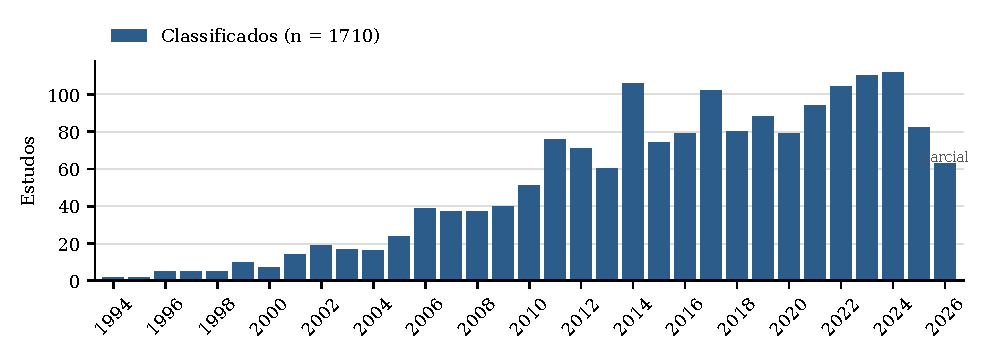
\includegraphics[width=\textwidth]{figs/years_pt.pdf}
\caption{Estudos incluídos por ano de publicação ($n = 456$).}\label{fig:years}
\end{figure}

A composição da área mudou bruscamente por volta de 2014 (Figura~\ref{fig:bubble}). Até 2013, o corpus é dominado por modelos estocásticos: 92\% dos estudos classificados de 1994--2005 e 73\% dos de 2006--2013 têm \ST{}. A partir de 2014, a mineração de processos assume a liderança, com \PM{} em 61\% dos estudos de 2014--2019 e em 60\% dos de 2020--2026, enquanto \ST{} cai para cerca de um terço. A mineração de repositórios (\MSR{}) cresce de forma contínua, de 3\% para 41\% dos estudos de cada período. A participação da previsão (\FC{}) permanece aproximadamente estável, entre 24\% e 35\%.

\begin{figure}[t]
\centering
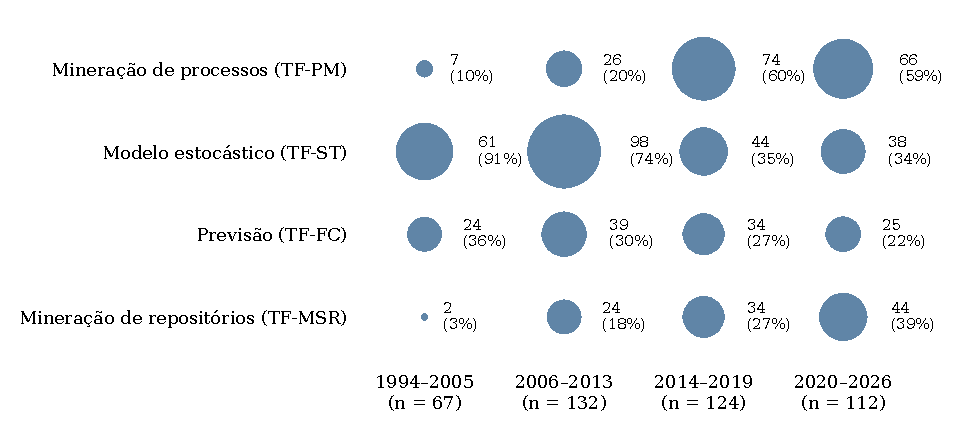
\includegraphics[width=0.92\textwidth]{figs/bubble_pt.pdf}
\caption{Famílias de técnica e de dados por período (estudos classificados, $n = 380$). A área de cada bolha é proporcional ao número de estudos; o percentual é a parcela dos estudos classificados do período que têm a família. As famílias não são mutuamente exclusivas.}\label{fig:bubble}
\end{figure}

\pendente{Acrescentar a distribuição por tipo de publicação (periódico, conferência, workshop) e os venues mais frequentes, a partir da extração da Seção~\ref{sec:classification}.}

\subsection{RQ2: Famílias de técnica e suas combinações}\label{sec:rq2}

Dos 380 estudos classificados, 210 (55,3\%) têm \ST{}, 157 (41,3\%) \PM{}, 111 (29,2\%) \FC{} e 97 (25,5\%) \MSR{}. A Tabela~\ref{tab:combos} mostra como as três famílias de técnica se combinam.

\begin{table}[t]
\centering\small
\caption{Combinações das três famílias de técnica nos 380 estudos classificados. Cada estudo aparece em exatamente uma linha. A coluna \MSR{} conta os estudos da linha que também mineram repositórios.}\label{tab:combos}
\begin{tabular}{lrrrc}
\toprule
Combinação & Estudos & \% & com \MSR{} & Ano mediano \\
\midrule
Apenas \PM{} & 141 & 37,1 & 62 & 2018 \\
Apenas \ST{} & 111 & 29,2 & 16 & 2008 \\
\ST{} + \FC{} & 89 & 23,4 & 2 & 2010 \\
Apenas \FC{} & 15 & 3,9 & 5 & 2019 \\
\PM{} + \ST{} & 9 & 2,4 & 1 & 2016 \\
Nenhuma (apenas \MSR{}) & 8 & 2,1 & 8 & 2017 \\
\PM{} + \FC{} & 6 & 1,6 & 3 & 2018 \\
\PM{} + \ST{} + \FC{} & 1 & 0,3 & 0 & 2025 \\
\midrule
Total & 380 & 100,0 & 97 & \\
\bottomrule
\end{tabular}
\end{table}

Dois agrupamentos respondem por 90\% do corpus e quase não se sobrepõem. O primeiro é a mineração de processos, frequentemente sobre dados de repositório: 141 estudos usam PM sem modelagem estocástica nem previsão, e 62 deles mineram repositórios. O segundo é a modelagem estocástica, isolada (111) ou usada para prever (89), quase nunca sobre eventos minerados de repositórios (18 de 200).

\paragraph{Mineração de processos}
O arco seminal de \PM{} vai da descoberta, por Cook e Wolf, de modelos de processo de estados finitos a partir de rastros de eventos, que já usava modelos de Markov~\cite{cook1995,cook1998}, à aplicação, por Rubin et al., do framework ProM a logs de gerência de código-fonte~\cite{rubin2007}. Trabalhos posteriores estenderam a descoberta a múltiplos repositórios e perspectivas.

\paragraph{Modelagem estocástica}
Os estudos com cadeias de Markov representam processos de software como transições discretas de estado: a atividade de desenvolvedores em repositórios GitHub como cadeias de Markov de tempo discreto~\cite{jo2023}, com verificação probabilística de modelos para propriedades temporais~\cite{jo2024}; padrões de inserção e de correção de falhas combinados com análise de redes sociais~\cite{ortu2023}; processos de decisão de Markov para predição do resultado de pull requests~\cite{joshi2024}; predição de risco a partir de dados de repositório~\cite{jeon2015}; remoção de defeitos sob \emph{code churn}~\cite{tian2005}; planejamento ágil em espaço de estados~\cite{tyagi2021}; previsão do momento de release~\cite{washizaki2015}; e estimativa de equipes com redes de autômatos estocásticos~\cite{massitela2018}. Redes de Petri estocásticas modelam a concorrência em pipelines de DevOps e de CI/CD~\cite{mesmia2021} e as etapas gargalo que governam a probabilidade de entrega~\cite{bhadra2022,bhadra2023}. A simulação de Monte Carlo apoia a previsão de projetos em modelos híbridos de dinâmica de sistemas~\cite{li2020}, a avaliação de riscos em métodos ágeis~\cite{lunesu2021} e a análise econômica do tempo de ciclo~\cite{magennis2015}.

Nesses estudos, probabilidades de transição, taxas de disparo e parâmetros de distribuições vêm de estatísticas agregadas de projeto, como contagens de defeitos, médias de duração por fase ou métricas de velocidade~\cite{nafreen2020,bhadra2022,li2020}. Os estados ficam ancorados em fases genéricas do ciclo de vida. Nenhum dos estudos citados deriva seu espaço de estados de um modelo de processo descoberto a partir de logs de eventos de granularidade fina.

\subsection{RQ3: Fases do SDLC, fontes de logs de eventos e técnicas}\label{sec:rq3}

\pendente{Esta subseção depende da extração humana (Seção~\ref{sec:classification}). Estrutura sugerida: (a) Tabela de fase do SDLC $\times$ família; (b) Tabela de fontes de event log (Jira, GitHub, GitLab, Jenkins, IDE, outras) e modo de construção; (c) frequência dos algoritmos de PM (Alpha, Heuristics, Inductive Miner, Fuzzy etc.), métodos estocásticos (DTMC, CTMC, SPN, Monte Carlo, System Dynamics) e alvos de previsão (lead time, remaining time, resolução de issue, outcome); (d) mapa de bolhas fase $\times$ família, como na Figura~\ref{fig:bubble}.}

\begin{table}[h]
\centering\small
\caption{\textcolor{red}{[PENDENTE]} Fases do SDLC abordadas, por família de técnica (estudos classificados). Um estudo pode abordar várias fases.}\label{tab:phases}
\begin{tabular}{lcccc}
\toprule
Fase do SDLC & \PM{} & \ST{} & \FC{} & \MSR{} \\
\midrule
Requisitos e projeto & -- & -- & -- & -- \\
Desenvolvimento (commits, pull requests) & -- & -- & -- & -- \\
Qualidade (teste, revisão, defeitos) & -- & -- & -- & -- \\
Entrega (CI/CD, release) & -- & -- & -- & -- \\
Operação (incidentes, manutenção) & -- & -- & -- & -- \\
\bottomrule
\end{tabular}
\end{table}

\subsection{RQ4: Integração e lacunas}\label{sec:rq4}

A Tabela~\ref{tab:levels} apresenta os níveis de integração. A maioria dos estudos (72,4\%) usa uma única família de técnica; 104 combinam duas; um combina três; nenhum atinge L3.

\begin{table}[t]
\centering\small
\caption{Níveis de integração dos 380 estudos classificados.}\label{tab:levels}
\begin{tabularx}{\textwidth}{lXrr}
\toprule
Nível & Definição & Estudos & \% \\
\midrule
L0 & No máximo uma família de técnica & 275 & 72,4 \\
L1 & Duas famílias de técnica (\PM{}+\ST{} 9; \PM{}+\FC{} 6; \ST{}+\FC{} 89) & 104 & 27,4 \\
L2 & Três famílias; etapas avaliadas separadamente & 1 & 0,3 \\
L3 & Três famílias acopladas por interfaces especificadas, avaliadas de ponta a ponta & 0 & 0,0 \\
\midrule
Total & & 380 & 100,0 \\
\bottomrule
\end{tabularx}
\end{table}

\paragraph{Mineração de processos com modelagem estocástica}
Dez estudos combinam \PM{} e \ST{}, oito deles publicados a partir de 2014. Eles acoplam a estrutura de processo descoberta a raciocínio estocástico para uma única questão analítica. Incerto et al.\ mostram que cadeias de Markov de comprimento variável superam dezoito técnicas de verificação de conformidade estocástica em dez de onze logs de \emph{benchmark}~\cite{incerto2025}. López-Pintado e Dumas substituem calendários determinísticos de recursos por calendários probabilísticos descobertos a partir de logs de eventos, reproduzindo com mais fidelidade as distribuições empíricas de tempo de ciclo~\cite{lopezpintado2023}. Jalote e Kamma modelam sequências de tarefas de programadores, extraídas de logs de IDE, como cadeias de Markov de primeira ordem~\cite{jalote2021}. Nenhum desses estudos usa a camada estocástica para prever uma métrica de processo.

\paragraph{Mineração de processos com previsão}
Sete estudos combinam \PM{} e \FC{}, todos publicados a partir de 2015. Eles abordam a predição por meio do aprimoramento de processos, e não de um modelo estocástico explícito. Gupta combina a descoberta com o \emph{inductive miner} e análise preditiva para identificar padrões recorrentes de falha em fluxos de manutenção~\cite{gupta2017}. O SIMPT extrai árvores de processo anotadas com tempo para simulação interativa do tipo ``e se''~\cite{pourbafrani2021}, linha estendida com modelos generativos~\cite{buliga2025}. Caldeira et al.\ derivam métricas de complexidade de processo a partir de logs de IDE e as usam para prever a qualidade do produto~\cite{caldeira2022}. Nenhum relata uma distribuição de probabilidade sobre o tempo de conclusão ou os passos restantes de uma instância individual de processo.

\paragraph{O único estudo com três famílias}
O PRIMAD~\cite{guinea2025} constrói um gêmeo digital do SDLC a partir de fluxos de issues do Jira, combinando descoberta baseada no pm4py, um núcleo de simulação baseado em atores e aprendizado supervisionado para predição sensível ao contexto. Sua avaliação é relatada por componente: o pipeline acoplado não é avaliado como um todo, as passagens entre etapas não são especificadas e nenhuma camada de previsão propaga a incerteza de ponta a ponta. Por isso, classificamos o estudo como L2.

\pendente{Registrar quem leu o PDF completo do PRIMAD e citar os trechos (seção/página) que mostram a avaliação por componente. Como a conclusão principal se apoia neste estudo, o revisor vai pedir isso.}

\paragraph{Lacunas}
Três lacunas decorrem das Tabelas~\ref{tab:combos} e~\ref{tab:levels}. Primeiro, a lacuna é de integração, não de cobertura: cada família está bem representada, mas as linhas de PM e estocástica se encontram em 10 de 380 estudos. Segundo, a previsão é feita sobretudo com modelos estocásticos alimentados por estatísticas agregadas (89 estudos) e raramente com estrutura minerada de logs de eventos (7). Terceiro, nenhum estudo avalia um pipeline de múltiplas etapas de ponta a ponta em dados do SDLC.

% =================================================================
\section{Discussão}\label{sec:discussion}

\subsection{Duas comunidades, uma fonte de dados}

O padrão mais nítido do corpus é a sucessão de duas comunidades sobre o mesmo tipo de dado. A modelagem estocástica de processos de software, com raízes na engenharia de confiabilidade e na simulação de processos, domina as duas primeiras décadas. A mineração de processos, com raízes na gestão de processos de negócio, domina a última e usa cada vez mais dados de repositório. Seus métodos são complementares: a PM fornece uma estrutura fundamentada empiricamente, e os modelos estocásticos fornecem distribuições sobre caminhos e durações. Ainda assim, o corpus contém poucos estudos que usam uma para alimentar a outra. Os estudos de PM com modelagem estocástica que encontramos vêm sobretudo do lado de processos de negócio e são avaliados em logs genéricos de \emph{benchmark}~\cite{incerto2025,lopezpintado2023}, linha que a literatura de mineração estocástica de processos dá continuidade~\cite{burke2020}.

\subsection{Agenda de pesquisa}\label{sec:agenda}

\begin{description}
\item[RA1.] \textbf{Construção padronizada de logs de eventos para o SDLC.} \emph{Frameworks} que transformem dados heterogêneos de repositório em logs de eventos comparáveis, com correlação de casos entre ferramentas. No corpus, os modelos de Markov da atividade em repositórios definem seus estados manualmente e de forma diferente a cada estudo~\cite{jo2023,jo2024,ortu2023}. \pendente{fundamentar com a contagem da Tabela de fontes e construção de logs (RQ3).}
\item[RA2.] \textbf{Previsão estocástica orientada a processos.} Derivar o espaço de estados e as probabilidades de transição de um modelo estocástico de previsão a partir de um modelo de processo descoberto, em vez de estatísticas agregadas. Esta é a combinação menos explorada (\PM{}+\ST{}: 10 estudos, nenhum prevendo uma métrica de processo).
\item[RA3.] \textbf{Atributos derivados de processos para preditores aprendidos.} Uso sistemático de atributos de conformidade, retrabalho e entropia de caminhos em preditores de engenharia de software, direção sugerida por~\cite{caldeira2022,gupta2017}. \pendente{fundamentar com a extração de RQ3 ou mover para trabalho futuro.}
\item[RA4.] \textbf{Benchmarks de ponta a ponta.} \emph{Benchmarks} abertos e compartilhados de código aberto, com separação temporal dos dados de teste, para que pipelines de múltiplas etapas possam ser comparados como um todo, e não por componente (L2 $\rightarrow$ L3).
\end{description}

\pendente{Taxonomia SPMF: aplicá-la aos 380 estudos (Analytical Depth $\times$ SDLC Coverage $\times$ Technique Integration), com mapa de bolhas, e reinserir aqui. Se não for aplicada, deixá-la só como proposta de trabalho futuro em uma frase, ou retirar.}

\subsection{Implicações para profissionais}

As técnicas do corpus operam sobre logs que já existem em rastreadores de issues e em controle de versão; assim, o custo de entrada está na construção dos logs de eventos, e não na coleta de dados. Nenhum estudo relata um pipeline de ponta a ponta avaliado como um único sistema. Um profissional que hoje encadeie PM, um modelo estocástico e um corretor aprendido estará combinando partes testadas individualmente cujo comportamento conjunto é desconhecido.

% =================================================================
\section{Ameaças à Validade}\label{sec:threats}

\subsection{Busca}\label{sec:threats-search}

As strings podem deixar de recuperar estudos que usam terminologia não canônica. A string complementar de MSR, a string de fronteira e a busca por citações atenuam esse risco. A verificação com o conjunto de controle é uma evidência fraca de completude: os dez estudos de controle já eram conhecidos quando as strings foram escritas, e três strings do Scopus incluem literalmente os títulos de estudos de controle. As strings não contêm bloco para previsão por aprendizado de máquina em dados de repositório; por isso, estudos que preveem métricas de processo com aprendizado de máquina sem termos de PM ou estocásticos estão sub-representados, e a participação de \FC{} provavelmente está subestimada. A revisão se limita a publicações em inglês revisadas por pares; literatura cinzenta, teses e preprints não foram pesquisados. As exportações do IEEE Xplore foram feitas em lotes manuais cuja string de origem não foi registrada.

\subsection{Seleção}

A primeira triagem usou um modelo de linguagem. O Recall do modelo na amostra verificada por humanos (0,630) ficou abaixo do critério predefinido de 0,90. Grande parte desse déficit vem da informação disponível para o modelo, e não do modelo em si: para 72,4\% dos registros do lote principal, a primeira decisão foi tomada apenas com o título, porque a exportação do Scopus não trazia resumos, e a segunda passagem leu o PDF em 0,5\% dos registros. O modelo foi executado com a temperatura padrão da API, de modo que suas decisões não são determinísticas. Por essas razões, a primeira triagem foi usada apenas para ordenar o trabalho, e todo registro que ela não incluiu foi triado novamente por humanos. A ameaça residual está nessa re-triagem humana: a concordância entre os revisores foi moderada na amostra do segundo lote ($\kappa = 0{,}494$), e os revisores viam rótulos sugeridos durante a triagem, o que pode ancorar suas decisões.

\subsection{Classificação}

Os códigos de família das inclusões originais foram propostos pelo modelo de linguagem e revisados pelos autores em todo estudo com duas famílias; os estudos de família única não foram auditados, de modo que um estudo com uma família não detectada pode estar subclassificado. Setenta e seis estudos não estão classificados. Se dois deles combinassem as três famílias, a contagem de L2 mudaria; um estudo L3 entre eles mudaria a conclusão principal. O julgamento entre L2 e L3 depende da leitura de um único estudo.

\subsection{Construto}

IC4b e IC4c admitem modelos de uso Markovianos para teste estatístico e modelos de crescimento de confiabilidade baseados em taxas de defeitos. Esses modelos descrevem o produto, e não o processo de desenvolvimento, e provavelmente respondem por muitos dos 89 estudos \ST{}+\FC{} de 1997--2013. Os autores desenvolvem um pipeline integrado de previsão; para limitar a influência desse interesse, os níveis de integração são definidos por critérios genéricos, e a referência ao nome do projeto dos autores no prompt do modelo de linguagem está declarada no pacote de replicação.

% =================================================================
\section{Conclusão}\label{sec:conclusion}

Mapeamos 456 estudos que aplicam mineração de processos, modelagem estocástica ou previsão a dados de desenvolvimento de software. A área foi moldada por duas comunidades em sucessão: a modelagem estocástica até 2013 e a mineração de processos desde 2014. Elas se encontram em 10 dos 380 estudos classificados. A previsão é feita sobretudo com modelos estocásticos alimentados por estatísticas agregadas, e raramente com estrutura de processo minerada de logs de eventos. Um estudo combina as três famílias, com cada componente avaliado separadamente; nenhum as acopla por meio de interfaces especificadas e avaliadas de ponta a ponta. A lacuna é, portanto, de integração, e não de técnicas disponíveis. A previsão estocástica orientada a processos e os \emph{benchmarks} de ponta a ponta são as duas direções com apoio mais claro no corpus.

O corpus, a classificação, os prompts e os registros de triagem estão disponíveis no pacote de replicação (Zenodo, DOI 10.5281/zenodo.21939600).

% =================================================================
\section*{Declaração de contribuição dos autores (CRediT)}
\textbf{Rodrigo Almeida de Oliveira:} Conceitualização, Metodologia, Software, Investigação, Curadoria de dados, Análise formal, Visualização, Escrita -- rascunho original, Escrita -- revisão e edição.
\textbf{Juliano de Paulo Ribeiro:} Metodologia, Validação, Investigação, Escrita -- revisão e edição.
\textbf{Edson Emilio Scalabrin:} Conceitualização, Metodologia, Supervisão, Escrita -- revisão e edição, Recursos, Obtenção de financiamento.

\section*{Declaração de conflito de interesses}
Os autores declaram não ter interesses financeiros concorrentes ou relações pessoais conhecidas que possam ter influenciado o trabalho relatado neste artigo.

\section*{Financiamento}
Este estudo foi financiado em parte pela Coordenação de Aperfeiçoamento de Pessoal de Nível Superior -- Brasil (CAPES) -- Código de Financiamento 001, por meio de bolsa de doutorado concedida ao autor correspondente no Programa de Pós-Graduação em Informática da Pontifícia Universidade Católica do Paraná (PPGIa/PUCPR).

\section*{Declaração sobre IA generativa no processo de escrita}
Durante a preparação deste trabalho, os autores usaram o Claude (Anthropic) para reestruturar e editar o manuscrito e para verificar sua aritmética. Após o uso dessa ferramenta, os autores revisaram e editaram o conteúdo conforme necessário e assumem total responsabilidade pelo conteúdo da publicação. Separadamente, um modelo de linguagem foi usado na condução do estudo como apoio à primeira triagem (Seção~\ref{sec:selection-process}).

\section*{Disponibilidade de dados}
O pacote de replicação (Zenodo, DOI 10.5281/zenodo.21939600) contém as strings de busca, os scripts de remoção de duplicatas e de enriquecimento, os prompts e esquemas de triagem, as decisões por registro em todas as etapas, as planilhas de verificação e de re-triagem humanas, a lista dos estudos incluídos com sua classificação e o checklist SEGRESS preenchido.
\pendente{Renomear \texttt{included\_studies\_506.csv} para \texttt{included\_studies.csv} e incluir \texttt{figs.py} e \texttt{studies.json} no pacote.}

\appendix

\section{Listas de termos de busca}\label{app:strings}

As strings são reproduzidas no idioma em que foram executadas.

\paragraph{String principal (população $\wedge$ intervenção)}
\begin{footnotesize}\begin{verbatim}
("software engineering" OR "software development" OR "software process"
 OR "software lifecycle" OR "software life cycle" OR "SDLC"
 OR "development lifecycle" OR "development life cycle" OR "DevOps"
 OR "CI/CD" OR "continuous integration" OR "continuous delivery"
 OR "agile development" OR "agile process" OR "issue tracking"
 OR "bug tracking" OR "version control" OR "code review" OR "pull request"
 OR "software project" OR "software repository" OR "software maintenance"
 OR "software evolution")
AND
("process mining" OR "process discovery" OR "conformance checking"
 OR "workflow mining" OR "predictive process monitoring"
 OR "process prediction" OR "remaining time prediction"
 OR "process forecasting" OR "event log" OR "process simulation"
 OR "Monte Carlo simulation" OR "Markov chain" OR "Markov model"
 OR "stochastic process model" OR "transition probability"
 OR "absorbing chain" OR "lead time prediction" OR "cycle time prediction")
\end{verbatim}\end{footnotesize}

\paragraph{String complementar (MSR $\rightarrow$ modelagem de processos)}
\begin{footnotesize}\begin{verbatim}
("mining software repositories" OR "software repository mining"
 OR "GitHub mining" OR "Jira mining")
AND ("process model" OR "Markov" OR "Monte Carlo" OR "stochastic"
 OR "lead time" OR "cycle time" OR "throughput" OR "transition matrix")
\end{verbatim}\end{footnotesize}

\paragraph{String de fronteira (estocástico $\wedge$ PM $\wedge$ ES)}
\begin{footnotesize}\begin{verbatim}
("Monte Carlo" OR "Markov chain" OR "stochastic simulation"
 OR "probabilistic forecast" OR "transition matrix")
AND ("process mining" OR "event log" OR "workflow mining"
 OR "process model" OR "business process")
AND ("software development" OR "software engineering" OR "software process"
 OR "DevOps" OR "SDLC" OR "issue tracker" OR "commit log"
 OR "build pipeline")
\end{verbatim}\end{footnotesize}

\section{Estudos incluídos}\label{app:studies}
\scriptsize
\setlength{\tabcolsep}{2.5pt}
\begin{longtable}{lll@{\hspace{10pt}}lll@{\hspace{10pt}}lll}
\caption{Os 1710 estudos incluídos (identificador no pacote de replicação, ano de publicação, famílias de técnica e de dados). PM = TF-PM, ST = TF-ST, FC = TF-FC, MSR = TF-MSR; $^{a}$ = acrescentado após o corpus-base (re-triagem humana, bloco ML da Fase~3, snowballing ou flips F2.3).}\label{tab:studies}\\
\toprule
ID & Year & Families & ID & Year & Families & ID & Year & Families \\
\midrule
\endfirsthead
\toprule
ID & Year & Families & ID & Year & Families & ID & Year & Families \\
\midrule
\endhead
\midrule
\multicolumn{9}{r}{Continued on next page}\\
\endfoot
\bottomrule
\endlastfoot
23068d2c & 1994 & ST$^{a}$ & c7a601d8 & 1994 & ST$^{a}$ & 520023e9 & 1995 & FC$^{a}$ \\
87bce30b & 1995 & PM+ST & 2225ebb5 & 1996 & FC$^{a}$ & 6d68591e & 1996 & PM \\
eec839f7 & 1996 & FC$^{a}$ & f9034283 & 1996 & FC$^{a}$ & ff339f4b & 1996 & FC$^{a}$ \\
421b3545 & 1997 & FC$^{a}$ & 50144afd & 1997 & ST+FC & 6115d05e & 1997 & ST$^{a}$ \\
8dea6481 & 1997 & ST$^{a}$ & be7c6454 & 1997 & PM+ST$^{a}$ & 07e55287 & 1998 & PM+ST \\
12f7f992 & 1998 & ST+FC$^{a}$ & 3f8fd941 & 1998 & ST+FC & 7f0d4fb9 & 1998 & FC$^{a}$ \\
85002ffb & 1998 & ST$^{a}$ & 17384cba & 1999 & FC$^{a}$ & 20a00ebf & 1999 & FC$^{a}$ \\
28685daa & 1999 & FC$^{a}$ & 66d00b19 & 1999 & ST+FC & afd1b7aa & 1999 & ST+FC \\
b24b55e3 & 1999 & ST$^{a}$ & d044ef55 & 1999 & ST & eb05417e & 1999 & ST \\
eb526806 & 1999 & PM & f453a92f & 1999 & ST & 072ba70b & 2000 & FC$^{a}$ \\
46287754 & 2000 & ST+FC & 9c255853 & 2000 & ST & a4f13cb1 & 2000 & ST+FC \\
ab16b112 & 2000 & ST & e82e259b & 2000 & ST$^{a}$ & f06ebc31 & 2000 & ST \\
19b34231 & 2001 & FC$^{a}$ & 39e47477 & 2001 & ST+FC & 4155a4da & 2001 & ST \\
49233222 & 2001 & FC$^{a}$ & 50dda3a0 & 2001 & ST+FC & 5e48a99f & 2001 & FC$^{a}$ \\
72329237 & 2001 & ST$^{a}$ & 839d520d & 2001 & ST+FC & 8ae72547 & 2001 & ST+FC \\
b48dde83 & 2001 & ST & da2f44fa & 2001 & ST+FC & e24af4e7 & 2001 & ST$^{a}$ \\
e516f339 & 2001 & FC$^{a}$ & f33d3c89 & 2001 & ST & 0743f004 & 2002 & FC$^{a}$ \\
0b759736 & 2002 & ST & 1703f629 & 2002 & FC$^{a}$ & 181f6213 & 2002 & FC$^{a}$ \\
363027c4 & 2002 & ST$^{a}$ & 743dcc43 & 2002 & PM+ST$^{a}$ & 7f8d2b91 & 2002 & PM$^{a}$ \\
86be15b0 & 2002 & FC$^{a}$ & 883e1702 & 2002 & ST+FC & 92f75feb & 2002 & FC$^{a}$ \\
a12f49f1 & 2002 & FC$^{a}$ & ad4f84a7 & 2002 & ST+MSR & b1aabe94 & 2002 & ST+FC \\
b75d202e & 2002 & ST+FC & c3e17c90 & 2002 & FC$^{a}$ & dcf53abb & 2002 & ST$^{a}$ \\
e3a9143c & 2002 & ST$^{a}$ & e620e55e & 2002 & ST$^{a}$ & f9c9914d & 2002 & FC$^{a}$ \\
0cb1d54a & 2003 & FC$^{a}$ & 1c928aae & 2003 & PM$^{a}$ & 3487bbf5 & 2003 & ST$^{a}$ \\
368dc22f & 2003 & ST$^{a}$ & 39157e2c & 2003 & ST & 3d0b754c & 2003 & FC$^{a}$ \\
46598602 & 2003 & FC$^{a}$ & 4b4df702 & 2003 & FC$^{a}$ & 4d84ffd3 & 2003 & FC$^{a}$ \\
4deba73b & 2003 & FC$^{a}$ & 6b16f9de & 2003 & ST$^{a}$ & 6e4114dc & 2003 & ST+FC \\
78969f65 & 2003 & ST & c35d9539 & 2003 & FC$^{a}$ & cda3f627 & 2003 & ST$^{a}$ \\
e9686368 & 2003 & ST$^{a}$ & ebc6dbac & 2003 & FC$^{a}$ & 1a7dfc0f & 2004 & FC$^{a}$ \\
25b10497 & 2004 & FC$^{a}$ & 3c810db6 & 2004 & ST & 46540576 & 2004 & ST$^{a}$ \\
58996946 & 2004 & ST & 5ba78162 & 2004 & FC$^{a}$ & 6408e693 & 2004 & PM+ST$^{a}$ \\
64c03c8d & 2004 & ST+FC & 7f2dd217 & 2004 & FC$^{a}$ & 9e8d5d7d & 2004 & FC$^{a}$ \\
a05aee89 & 2004 & FC$^{a}$ & ab99a53e & 2004 & PM+MSR & b37c10c1 & 2004 & ST+FC \\
c03603a2 & 2004 & FC$^{a}$ & c9512bbb & 2004 & ST+FC & fd7ca261 & 2004 & ST$^{a}$ \\
0232276d & 2005 & ST$^{a}$ & 11258fed & 2005 & FC$^{a}$ & 190c11c4 & 2005 & ST$^{a}$ \\
2fbf6d36 & 2005 & ST+FC & 33361b00 & 2005 & ST$^{a}$ & 3cc5a1cb & 2005 & ST \\
41a0e151 & 2005 & FC$^{a}$ & 48275fa8 & 2005 & FC$^{a}$ & 486ca310 & 2005 & FC$^{a}$ \\
4a2d3698 & 2005 & FC$^{a}$ & 557b4102 & 2005 & ST & 5b51a065 & 2005 & ST \\
6d37f6fe & 2005 & FC$^{a}$ & 6d83b874 & 2005 & ST+FC$^{a}$ & 74a9a45a & 2005 & FC$^{a}$ \\
7bebca2e & 2005 & FC$^{a}$ & 81929ce8 & 2005 & FC$^{a}$ & 88c18a84 & 2005 & ST$^{a}$ \\
a20e7c58 & 2005 & ST+FC & a27f51ca & 2005 & FC$^{a}$ & c94fc209 & 2005 & ST+FC \\
d67f1905 & 2005 & FC$^{a}$ & f330dbc0 & 2005 & FC$^{a}$ & ff1faf6c & 2005 & FC+MSR$^{a}$ \\
063967eb & 2006 & ST+FC$^{a}$ & 117db759 & 2006 & ST$^{a}$ & 24059629 & 2006 & ST$^{a}$ \\
2c280053 & 2006 & PM+MSR & 307385ce & 2006 & FC$^{a}$ & 35cf3bbf & 2006 & FC$^{a}$ \\
3c2136fd & 2006 & FC$^{a}$ & 416c979c & 2006 & ST+FC & 48e69187 & 2006 & PM+MSR \\
53434e77 & 2006 & ST+MSR & 66c95d97 & 2006 & ST$^{a}$ & 6795e33c & 2006 & ST$^{a}$ \\
72bbaa1b & 2006 & FC$^{a}$ & 74accbf5 & 2006 & FC$^{a}$ & 7766e7b4 & 2006 & ST \\
78f76ab8 & 2006 & FC$^{a}$ & 836b5ef0 & 2006 & ST+FC & 8888cfdc & 2006 & ST \\
8e0eec4d & 2006 & ST+FC & 9eff3fd0 & 2006 & FC$^{a}$ & 9f8b9dba & 2006 & ST+MSR \\
a9dd0444 & 2006 & FC$^{a}$ & abc76a20 & 2006 & FC$^{a}$ & ae4f4926 & 2006 & ST \\
b5b1402b & 2006 & ST+FC & b5b6fcff & 2006 & FC$^{a}$ & b78523e4 & 2006 & PM$^{a}$ \\
bd8b607e & 2006 & FC$^{a}$ & be942093 & 2006 & PM & c3683c28 & 2006 & PM+MSR \\
c89287f2 & 2006 & FC$^{a}$ & cb6e46b8 & 2006 & FC$^{a}$ & cdf1f104 & 2006 & PM+MSR \\
d50fcf26 & 2006 & ST & dbcd2435 & 2006 & ST+FC & dc9483c1 & 2006 & FC$^{a}$ \\
df3ad75a & 2006 & PM+MSR & ec94ba4d & 2006 & ST+FC & fe75ced8 & 2006 & ST$^{a}$ \\
0078a735 & 2007 & FC$^{a}$ & 0c5b4491 & 2007 & FC$^{a}$ & 0e12a280 & 2007 & FC$^{a}$ \\
16a201ed & 2007 & ST$^{a}$ & 171085b9 & 2007 & ST$^{a}$ & 19f6b59f & 2007 & FC$^{a}$ \\
228961c5 & 2007 & FC$^{a}$ & 261f9099 & 2007 & FC$^{a}$ & 30769647 & 2007 & FC$^{a}$ \\
3626fef4 & 2007 & ST$^{a}$ & 3ddbfd94 & 2007 & PM & 3ef9d4b3 & 2007 & FC$^{a}$ \\
57195f58 & 2007 & FC$^{a}$ & 632586c5 & 2007 & FC$^{a}$ & 65bbe771 & 2007 & FC$^{a}$ \\
747fc068 & 2007 & ST+FC & 8e41b716 & 2007 & PM$^{a}$ & 9870248b & 2007 & ST \\
a2bc654c & 2007 & FC$^{a}$ & a2d3ea2d & 2007 & FC$^{a}$ & a401497c & 2007 & ST$^{a}$ \\
a4ad0347 & 2007 & ST$^{a}$ & a887b16d & 2007 & FC$^{a}$ & aa0da064 & 2007 & ST+FC$^{a}$ \\
ac05d867 & 2007 & ST & d1f084f4 & 2007 & FC$^{a}$ & d7b22f54 & 2007 & ST \\
df9a3f24 & 2007 & FC$^{a}$ & e07c6819 & 2007 & MSR$^{a}$ & e9a40e7a & 2007 & ST \\
e9d3ec8a & 2007 & FC$^{a}$ & ee3f437e & 2007 & FC$^{a}$ & f2ba79cc & 2007 & FC$^{a}$ \\
faea5ac1 & 2007 & FC$^{a}$ & fba07e74 & 2007 & FC$^{a}$ & fc1caae7 & 2007 & FC$^{a}$ \\
fdd3425a & 2007 & FC$^{a}$ & 01c715f4 & 2008 & FC$^{a}$ & 070fae7f & 2008 & FC$^{a}$ \\
0fcd5ece & 2008 & ST & 2a8b96f3 & 2008 & FC$^{a}$ & 2d31d28f & 2008 & FC$^{a}$ \\
2fb4f513 & 2008 & ST & 37f008b1 & 2008 & FC$^{a}$ & 38625f3b & 2008 & ST$^{a}$ \\
38fae842 & 2008 & FC$^{a}$ & 3ae2f9fd & 2008 & ST$^{a}$ & 3c0dd1ad & 2008 & ST+FC \\
40bc718e & 2008 & ST & 4f530975 & 2008 & FC$^{a}$ & 52ee5271 & 2008 & FC$^{a}$ \\
58475e17 & 2008 & FC$^{a}$ & 5c43edc7 & 2008 & ST+FC & 6269e223 & 2008 & FC$^{a}$ \\
6f5e6f89 & 2008 & ST$^{a}$ & 7e6b3f9f & 2008 & PM & 861c4959 & 2008 & FC$^{a}$ \\
863bae01 & 2008 & ST+FC & 89fd72e8 & 2008 & FC$^{a}$ & 91493886 & 2008 & FC$^{a}$ \\
afb37589 & 2008 & FC$^{a}$ & b8b834e2 & 2008 & ST & ba328b1c & 2008 & ST$^{a}$ \\
cb68ba73 & 2008 & FC$^{a}$ & d8fc6aba & 2008 & FC$^{a}$ & deae809b & 2008 & ST+MSR \\
dfb2398b & 2008 & ST$^{a}$ & e080b18d & 2008 & ST+FC & e2d3c67e & 2008 & FC$^{a}$ \\
e5fa7505 & 2008 & ST$^{a}$ & e6075fca & 2008 & ST$^{a}$ & edd4c661 & 2008 & FC$^{a}$ \\
fb4a2cb3 & 2008 & ST+FC$^{a}$ & fbf7e330 & 2008 & ST$^{a}$ & 008caf63 & 2009 & ST+FC \\
0906c3aa & 2009 & ST$^{a}$ & 20795cca & 2009 & FC$^{a}$ & 2551d106 & 2009 & FC$^{a}$ \\
2d148576 & 2009 & FC$^{a}$ & 30ff5eac & 2009 & FC$^{a}$ & 31a8cb54 & 2009 & ST$^{a}$ \\
35d428b0 & 2009 & FC$^{a}$ & 3b4591cd & 2009 & ST+FC & 3e8a5f46 & 2009 & MSR$^{a}$ \\
47de5b9b & 2009 & FC$^{a}$ & 52c2c79d & 2009 & FC$^{a}$ & 5e847cf3 & 2009 & FC$^{a}$ \\
67b85117 & 2009 & ST+FC$^{a}$ & 6a71c8cc & 2009 & FC$^{a}$ & 70af8211 & 2009 & ST+FC \\
8f1fb42b & 2009 & ST$^{a}$ & 917f238d & 2009 & PM & 989891c5 & 2009 & ST$^{a}$ \\
a31937db & 2009 & FC$^{a}$ & a7ff3f61 & 2009 & FC$^{a}$ & a98f6c54 & 2009 & ST$^{a}$ \\
b2c57fd3 & 2009 & ST+FC & b594fa65 & 2009 & FC$^{a}$ & b80334f7 & 2009 & FC$^{a}$ \\
bd372642 & 2009 & FC$^{a}$ & beb83053 & 2009 & ST+FC & c0f6c7bd & 2009 & FC$^{a}$ \\
cfea47e6 & 2009 & FC$^{a}$ & d12bfa4c & 2009 & FC$^{a}$ & d43051f3 & 2009 & FC$^{a}$ \\
ddeca0e6 & 2009 & PM & df61a7a1 & 2009 & FC$^{a}$ & e1e6101d & 2009 & FC$^{a}$ \\
e856dbe4 & 2009 & PM+MSR & ee5ccaa2 & 2009 & PM & eeed2f5d & 2009 & ST$^{a}$ \\
fc8f325d & 2009 & ST+FC & fcc830f6 & 2009 & ST & fd5bab59 & 2009 & FC$^{a}$ \\
012922af & 2010 & FC$^{a}$ & 02e1bb05 & 2010 & FC$^{a}$ & 0ab0a53e & 2010 & FC$^{a}$ \\
0ef6a5b4 & 2010 & ST+FC & 15d941d7 & 2010 & FC$^{a}$ & 1cd3c3f0 & 2010 & FC$^{a}$ \\
1d754c2e & 2010 & ST$^{a}$ & 26582491 & 2010 & ST & 2bc341c0 & 2010 & FC$^{a}$ \\
3476b5db & 2010 & ST+FC & 36ada7be & 2010 & FC$^{a}$ & 3e19e5b7 & 2010 & FC$^{a}$ \\
4a85a963 & 2010 & FC$^{a}$ & 4f3ac568 & 2010 & FC$^{a}$ & 52756657 & 2010 & FC$^{a}$ \\
5357188e & 2010 & FC$^{a}$ & 53c06c4c & 2010 & FC$^{a}$ & 559a576d & 2010 & FC$^{a}$ \\
5f66b602 & 2010 & ST+FC$^{a}$ & 62936834 & 2010 & ST+FC & 6354fc81 & 2010 & ST+FC \\
6c5aae2a & 2010 & FC$^{a}$ & 7692b4f3 & 2010 & FC$^{a}$ & 7f497573 & 2010 & ST+FC \\
7f8fbfcd & 2010 & FC$^{a}$ & 839eaa6b & 2010 & FC$^{a}$ & 865b13e0 & 2010 & FC$^{a}$ \\
86d2ae2d & 2010 & FC$^{a}$ & 86f0c466 & 2010 & ST$^{a}$ & 937705ca & 2010 & FC$^{a}$ \\
939e52ff & 2010 & FC$^{a}$ & 980c26fa & 2010 & FC$^{a}$ & a210fdd3 & 2010 & ST$^{a}$ \\
a222ef2c & 2010 & PM+MSR & a5c1650b & 2010 & MSR$^{a}$ & a7082664 & 2010 & FC$^{a}$ \\
a7e713c2 & 2010 & FC$^{a}$ & a894367d & 2010 & FC$^{a}$ & afb8f80d & 2010 & FC$^{a}$ \\
b835ddc7 & 2010 & FC$^{a}$ & ba2ff831 & 2010 & ST & bafb58a0 & 2010 & PM+MSR \\
c113bf1b & 2010 & PM+MSR & c72f823c & 2010 & ST & ca22bfe7 & 2010 & ST$^{a}$ \\
cd860b9f & 2010 & ST$^{a}$ & d55dd861 & 2010 & FC$^{a}$ & d96a3161 & 2010 & PM+MSR \\
e93c382e & 2010 & FC$^{a}$ & f22983b3 & 2010 & FC$^{a}$ & ffe69110 & 2010 & FC$^{a}$ \\
0132f840 & 2011 & FC$^{a}$ & 04e0e983 & 2011 & ST$^{a}$ & 0b2f6ca9 & 2011 & FC$^{a}$ \\
104187af & 2011 & FC$^{a}$ & 155125ff & 2011 & FC$^{a}$ & 16ec93d7 & 2011 & ST$^{a}$ \\
18910ceb & 2011 & FC$^{a}$ & 1caa9a9e & 2011 & FC$^{a}$ & 1e4da643 & 2011 & FC$^{a}$ \\
1edfbbfa & 2011 & FC$^{a}$ & 2528f10d & 2011 & FC$^{a}$ & 266210a7 & 2011 & ST \\
27e504af & 2011 & FC$^{a}$ & 296c473a & 2011 & FC$^{a}$ & 2de8a9af & 2011 & FC \\
3155ca7a & 2011 & FC$^{a}$ & 32aacfa7 & 2011 & FC$^{a}$ & 35bcb278 & 2011 & ST+FC$^{a}$ \\
37582a83 & 2011 & FC$^{a}$ & 386325c8 & 2011 & FC$^{a}$ & 3d174d69 & 2011 & FC$^{a}$ \\
3f5f23a9 & 2011 & FC$^{a}$ & 4316248d & 2011 & PM & 460fa1fc & 2011 & FC$^{a}$ \\
47ed5bf0 & 2011 & ST+MSR & 4a072003 & 2011 & FC$^{a}$ & 4d088b6b & 2011 & ST$^{a}$ \\
4f2424db & 2011 & FC+MSR$^{a}$ & 51b4ae2b & 2011 & ST+FC & 576b8543 & 2011 & FC$^{a}$ \\
57d2445c & 2011 & ST+FC & 5c322411 & 2011 & FC$^{a}$ & 5c3f99ea & 2011 & ST$^{a}$ \\
5c86719e & 2011 & FC$^{a}$ & 5e335d0b & 2011 & FC$^{a}$ & 602d4cc6 & 2011 & ST$^{a}$ \\
6dbfdf97 & 2011 & FC$^{a}$ & 6e574443 & 2011 & FC$^{a}$ & 704a0d34 & 2011 & ST$^{a}$ \\
7206bd3c & 2011 & FC$^{a}$ & 7a18f4ee & 2011 & FC$^{a}$ & 7afcd1b2 & 2011 & FC+MSR$^{a}$ \\
7eaf7eb3 & 2011 & ST & 7fd7fade & 2011 & FC$^{a}$ & 84315802 & 2011 & ST \\
917d9592 & 2011 & ST & 93f4daf3 & 2011 & FC$^{a}$ & 986ed4b1 & 2011 & FC$^{a}$ \\
9ae84d72 & 2011 & PM$^{a}$ & 9f26ca4a & 2011 & FC$^{a}$ & a295c1b6 & 2011 & FC$^{a}$ \\
aaa79bcd & 2011 & FC$^{a}$ & b61ea92e & 2011 & ST+FC & bc57ea5b & 2011 & FC$^{a}$ \\
c24db118 & 2011 & PM & c4269b60 & 2011 & FC+MSR$^{a}$ & c4703958 & 2011 & FC$^{a}$ \\
c517c93f & 2011 & PM+MSR & c7682ec2 & 2011 & PM+MSR & c815bcc6 & 2011 & ST$^{a}$ \\
cafaba8c & 2011 & FC$^{a}$ & cccf4e66 & 2011 & FC$^{a}$ & ce92cc23 & 2011 & FC$^{a}$ \\
d098c91d & 2011 & PM & d556b5d1 & 2011 & FC$^{a}$ & d7bc3e1a & 2011 & FC$^{a}$ \\
de24553f & 2011 & FC$^{a}$ & debdebc2 & 2011 & ST$^{a}$ & e0cd71ab & 2011 & FC$^{a}$ \\
e39e4f39 & 2011 & FC$^{a}$ & e8e53811 & 2011 & FC$^{a}$ & ee504329 & 2011 & FC$^{a}$ \\
efab3f7f & 2011 & ST$^{a}$ & f047f55e & 2011 & FC$^{a}$ & f450a0aa & 2011 & FC$^{a}$ \\
f516d8b6 & 2011 & FC$^{a}$ & 0202e682 & 2012 & FC$^{a}$ & 03fd9dfc & 2012 & FC$^{a}$ \\
076d92c4 & 2012 & FC$^{a}$ & 0c10d633 & 2012 & ST+FC & 0d306f3b & 2012 & FC$^{a}$ \\
0e15e613 & 2012 & MSR$^{a}$ & 0e708ae8 & 2012 & MSR$^{a}$ & 1099ff04 & 2012 & FC$^{a}$ \\
1303e41e & 2012 & ST$^{a}$ & 1bfc6bec & 2012 & FC$^{a}$ & 1f3777ef & 2012 & FC$^{a}$ \\
21121cbf & 2012 & ST+MSR$^{a}$ & 214d17c4 & 2012 & ST$^{a}$ & 214efe16 & 2012 & FC$^{a}$ \\
23ec55bd & 2012 & ST & 2c7144d6 & 2012 & FC$^{a}$ & 2c7ec6c7 & 2012 & FC$^{a}$ \\
2f7a6894 & 2012 & FC+MSR$^{a}$ & 326da20f & 2012 & ST & 33cdea14 & 2012 & ST$^{a}$ \\
37bba7f6 & 2012 & FC$^{a}$ & 3ee20edf & 2012 & FC+MSR$^{a}$ & 3f09473c & 2012 & ST$^{a}$ \\
4634263a & 2012 & FC$^{a}$ & 46cbe525 & 2012 & FC$^{a}$ & 489b63cb & 2012 & FC$^{a}$ \\
4bc22efd & 2012 & FC$^{a}$ & 555f2c80 & 2012 & FC$^{a}$ & 5593f550 & 2012 & FC$^{a}$ \\
5aa1ae73 & 2012 & FC$^{a}$ & 5ae29e8c & 2012 & FC$^{a}$ & 5c7a03c0 & 2012 & FC$^{a}$ \\
5ffe33d2 & 2012 & FC$^{a}$ & 66a32124 & 2012 & ST+FC & 6c89be51 & 2012 & FC$^{a}$ \\
72fb141c & 2012 & FC+MSR$^{a}$ & 7453dad6 & 2012 & FC$^{a}$ & 79eac7e5 & 2012 & FC$^{a}$ \\
900def3d & 2012 & FC$^{a}$ & 984e32d4 & 2012 & FC$^{a}$ & a307e0c1 & 2012 & FC$^{a}$ \\
a3c061ae & 2012 & ST+FC & a8a3e15d & 2012 & FC$^{a}$ & ab9983cb & 2012 & FC$^{a}$ \\
ae20e68e & 2012 & PM & ae2ff7cf & 2012 & FC$^{a}$ & aea9f86e & 2012 & FC$^{a}$ \\
aef9dbee & 2012 & FC$^{a}$ & b58bf16e & 2012 & FC$^{a}$ & b888412a & 2012 & FC$^{a}$ \\
b8d51dfd & 2012 & FC$^{a}$ & b94c32dd & 2012 & FC$^{a}$ & bbc13de4 & 2012 & PM+MSR \\
bcce3152 & 2012 & FC$^{a}$ & bfe1fbcc & 2012 & FC$^{a}$ & c98ee85a & 2012 & FC$^{a}$ \\
c9ee07ba & 2012 & FC$^{a}$ & ca00050f & 2012 & ST+MSR & d3689e89 & 2012 & FC$^{a}$ \\
d4601a2f & 2012 & MSR & da28afcb & 2012 & ST$^{a}$ & dbc78b51 & 2012 & FC$^{a}$ \\
df22b7bc & 2012 & FC$^{a}$ & dfe889ba & 2012 & FC$^{a}$ & e6eada40 & 2012 & FC$^{a}$ \\
f27117e2 & 2012 & ST$^{a}$ & f311234a & 2012 & FC$^{a}$ & f5151d89 & 2012 & ST+FC \\
fa9fe762 & 2012 & FC$^{a}$ & fcbe1fac & 2012 & FC$^{a}$ & ff19d97c & 2012 & FC$^{a}$ \\
009af547 & 2013 & FC$^{a}$ & 0448f98d & 2013 & FC$^{a}$ & 050fa5cf & 2013 & ST$^{a}$ \\
09363023 & 2013 & FC$^{a}$ & 0d29ff1f & 2013 & FC$^{a}$ & 14dbc2fa & 2013 & FC$^{a}$ \\
17a4707b & 2013 & FC$^{a}$ & 18289398 & 2013 & FC$^{a}$ & 1f58d29f & 2013 & ST+FC$^{a}$ \\
203ec332 & 2013 & FC$^{a}$ & 264019f3 & 2013 & FC$^{a}$ & 2784f4ea & 2013 & FC$^{a}$ \\
2d93db80 & 2013 & FC$^{a}$ & 322484bf & 2013 & FC$^{a}$ & 3b614f91 & 2013 & ST+FC \\
3d6aeed8 & 2013 & MSR$^{a}$ & 40b67211 & 2013 & FC$^{a}$ & 43773183 & 2013 & ST$^{a}$ \\
455b830c & 2013 & FC$^{a}$ & 4ba174fc & 2013 & FC+MSR$^{a}$ & 4c5b8652 & 2013 & FC$^{a}$ \\
59919e44 & 2013 & FC$^{a}$ & 5b52b11e & 2013 & FC$^{a}$ & 5d5f0292 & 2013 & FC$^{a}$ \\
5f9bb212 & 2013 & FC$^{a}$ & 60e4fba6 & 2013 & MSR$^{a}$ & 6789e54a & 2013 & FC+MSR$^{a}$ \\
69230937 & 2013 & FC$^{a}$ & 81adcdde & 2013 & FC$^{a}$ & 81dd5091 & 2013 & FC$^{a}$ \\
84407144 & 2013 & FC$^{a}$ & 86c11e29 & 2013 & FC$^{a}$ & 88b8156e & 2013 & FC$^{a}$ \\
8ea2246c & 2013 & FC$^{a}$ & 9174f5b6 & 2013 & FC$^{a}$ & 95fbffdc & 2013 & FC$^{a}$ \\
97603c0b & 2013 & FC$^{a}$ & 9d553716 & 2013 & FC$^{a}$ & a257388d & 2013 & FC$^{a}$ \\
a8594e55 & 2013 & FC$^{a}$ & a8b7ed5a & 2013 & FC$^{a}$ & aeae5ed0 & 2013 & FC$^{a}$ \\
b4540e0e & 2013 & FC$^{a}$ & b66fac38 & 2013 & FC$^{a}$ & b721525d & 2013 & FC$^{a}$ \\
bd0d0222 & 2013 & FC$^{a}$ & c195758e & 2013 & FC$^{a}$ & cc3e46a9 & 2013 & FC$^{a}$ \\
cd17b2ad & 2013 & ST$^{a}$ & cd32f232 & 2013 & FC$^{a}$ & d2b57e47 & 2013 & FC+MSR$^{a}$ \\
d5665995 & 2013 & FC$^{a}$ & d892a8fb & 2013 & FC$^{a}$ & ddc8cc8c & 2013 & FC$^{a}$ \\
ecbed8c4 & 2013 & FC$^{a}$ & edb05739 & 2013 & FC$^{a}$ & edda2671 & 2013 & FC$^{a}$ \\
faa981c4 & 2013 & FC$^{a}$ & fdbc7853 & 2013 & FC$^{a}$ & fed24e09 & 2013 & FC$^{a}$ \\
01fba467 & 2014 & FC$^{a}$ & 024c9fcd & 2014 & FC$^{a}$ & 05ce7f00 & 2014 & FC$^{a}$ \\
0c80db13 & 2014 & FC$^{a}$ & 1282204f & 2014 & FC$^{a}$ & 1363926c & 2014 & ST+FC \\
149dedd4 & 2014 & FC$^{a}$ & 14bd5a7f & 2014 & FC$^{a}$ & 183b6bb9 & 2014 & ST+FC$^{a}$ \\
1de657c1 & 2014 & PM+MSR & 2099ce3a & 2014 & FC$^{a}$ & 229f1656 & 2014 & FC$^{a}$ \\
2365ec87 & 2014 & FC$^{a}$ & 25969842 & 2014 & FC$^{a}$ & 26b762ac & 2014 & FC$^{a}$ \\
27ca7b0a & 2014 & FC+MSR$^{a}$ & 2a7de581 & 2014 & ST+FC & 2f1e25da & 2014 & ST$^{a}$ \\
3231578f & 2014 & PM & 358ea1c9 & 2014 & FC$^{a}$ & 3726ebce & 2014 & FC$^{a}$ \\
3bd2d170 & 2014 & FC$^{a}$ & 3e13bdae & 2014 & FC$^{a}$ & 42e8f821 & 2014 & FC$^{a}$ \\
4748abd8 & 2014 & FC$^{a}$ & 477393d4 & 2014 & FC$^{a}$ & 49527f55 & 2014 & FC+MSR$^{a}$ \\
4aa53bdd & 2014 & FC$^{a}$ & 4cff6b4d & 2014 & PM+MSR & 4e2c29c1 & 2014 & FC$^{a}$ \\
4fc7fbfc & 2014 & FC$^{a}$ & 51450f2c & 2014 & FC$^{a}$ & 542728fe & 2014 & ST \\
55def679 & 2014 & FC$^{a}$ & 566e24e8 & 2014 & FC$^{a}$ & 586b96ab & 2014 & FC$^{a}$ \\
5a466249 & 2014 & FC$^{a}$ & 5a602862 & 2014 & FC+MSR$^{a}$ & 5d027dd1 & 2014 & FC$^{a}$ \\
5faae738 & 2014 & FC$^{a}$ & 5fc630db & 2014 & FC$^{a}$ & 5fe2fe46 & 2014 & ST$^{a}$ \\
68fb9a94 & 2014 & PM$^{a}$ & 6927a5a3 & 2014 & FC$^{a}$ & 6952fcb7 & 2014 & FC$^{a}$ \\
6b273691 & 2014 & FC$^{a}$ & 6f697869 & 2014 & FC$^{a}$ & 6fd30d7e & 2014 & PM+MSR \\
70c7203e & 2014 & FC$^{a}$ & 76e991ee & 2014 & FC+MSR$^{a}$ & 7ac425f7 & 2014 & FC$^{a}$ \\
7f7591d0 & 2014 & FC$^{a}$ & 7fdeb0fa & 2014 & FC$^{a}$ & 829f8c13 & 2014 & PM+MSR \\
88ee1d90 & 2014 & ST+FC$^{a}$ & 8c42d0fe & 2014 & PM$^{a}$ & 8c928c6a & 2014 & FC+MSR$^{a}$ \\
8cb831d9 & 2014 & FC$^{a}$ & 90ce9c17 & 2014 & FC$^{a}$ & 932f2a18 & 2014 & PM \\
98c7bb26 & 2014 & FC$^{a}$ & 99310b4c & 2014 & FC$^{a}$ & 9dd53fdd & 2014 & FC$^{a}$ \\
a13cfb0c & 2014 & FC$^{a}$ & a16b863d & 2014 & FC$^{a}$ & ad250ae5 & 2014 & PM \\
ad5c0b40 & 2014 & FC+MSR$^{a}$ & b117b377 & 2014 & FC$^{a}$ & b5a40ee4 & 2014 & FC$^{a}$ \\
b9b3d835 & 2014 & FC$^{a}$ & b9d7b3e8 & 2014 & FC$^{a}$ & bc871cea & 2014 & FC$^{a}$ \\
bcdd7b6f & 2014 & FC$^{a}$ & c1575581 & 2014 & FC$^{a}$ & c2dae430 & 2014 & FC$^{a}$ \\
c50ffd51 & 2014 & FC$^{a}$ & c6366ed4 & 2014 & FC$^{a}$ & c854882d & 2014 & FC$^{a}$ \\
c8e54484 & 2014 & FC$^{a}$ & c8ea828e & 2014 & PM & c9cdb64d & 2014 & PM \\
ce72fe95 & 2014 & FC$^{a}$ & cef0d2f7 & 2014 & FC$^{a}$ & d1ed6154 & 2014 & PM+MSR \\
d6b59a61 & 2014 & FC$^{a}$ & d6d61646 & 2014 & FC$^{a}$ & d82592db & 2014 & FC$^{a}$ \\
db3af2f6 & 2014 & FC$^{a}$ & defccca9 & 2014 & FC$^{a}$ & e032af1f & 2014 & FC$^{a}$ \\
e2533ddb & 2014 & FC$^{a}$ & e36fe110 & 2014 & FC$^{a}$ & e58074e0 & 2014 & PM \\
e69d723f & 2014 & PM$^{a}$ & e722b1cf & 2014 & PM+ST+MSR & e8daaada & 2014 & PM$^{a}$ \\
eb7732ed & 2014 & FC$^{a}$ & ed17c20e & 2014 & PM$^{a}$ & f01ab608 & 2014 & FC$^{a}$ \\
f1fc3f03 & 2014 & FC$^{a}$ & f27bbb48 & 2014 & FC$^{a}$ & f28af826 & 2014 & FC$^{a}$ \\
f3b5dc7a & 2014 & FC$^{a}$ & f6edde4a & 2014 & ST & fe09a77e & 2014 & FC$^{a}$ \\
fe225f50 & 2014 & FC+MSR$^{a}$ & 02f7a03b & 2015 & FC$^{a}$ & 02f96e2f & 2015 & FC$^{a}$ \\
058b73dc & 2015 & FC$^{a}$ & 05b677ed & 2015 & FC$^{a}$ & 087be32f & 2015 & FC$^{a}$ \\
0d56225b & 2015 & FC$^{a}$ & 12fbf63a & 2015 & ST$^{a}$ & 164bff33 & 2015 & FC$^{a}$ \\
18ed6f12 & 2015 & FC$^{a}$ & 1f99d374 & 2015 & FC$^{a}$ & 261f6383 & 2015 & ST+FC \\
2647ea07 & 2015 & PM & 27a05621 & 2015 & FC$^{a}$ & 2b497476 & 2015 & FC$^{a}$ \\
2ee3dc10 & 2015 & PM+MSR & 32027321 & 2015 & FC$^{a}$ & 328123bc & 2015 & PM+ST+FC$^{a}$ \\
329c586c & 2015 & FC$^{a}$ & 35f7dbe4 & 2015 & FC$^{a}$ & 3a39fa54 & 2015 & FC$^{a}$ \\
3ac74336 & 2015 & ST+FC & 3ad60828 & 2015 & FC$^{a}$ & 3ad9cd69 & 2015 & ST+FC \\
3d379233 & 2015 & PM+MSR & 405b5b88 & 2015 & FC$^{a}$ & 4b2c7904 & 2015 & FC+MSR$^{a}$ \\
4eeb076b & 2015 & PM+FC$^{a}$ & 508f3b5b & 2015 & PM & 5202932a & 2015 & PM$^{a}$ \\
582a391e & 2015 & FC$^{a}$ & 5af6706b & 2015 & PM$^{a}$ & 5d68fa29 & 2015 & FC$^{a}$ \\
5eba4c4b & 2015 & FC$^{a}$ & 605e3a34 & 2015 & FC+MSR$^{a}$ & 6069e7b2 & 2015 & FC$^{a}$ \\
769bbb49 & 2015 & FC+MSR$^{a}$ & 786d57aa & 2015 & ST$^{a}$ & 789cf287 & 2015 & FC$^{a}$ \\
7a242c5c & 2015 & FC$^{a}$ & 80efe394 & 2015 & FC+MSR$^{a}$ & 82b3401d & 2015 & PM \\
903cc52e & 2015 & FC$^{a}$ & 927817d5 & 2015 & ST+FC & 9611503c & 2015 & FC$^{a}$ \\
98875adb & 2015 & FC+MSR$^{a}$ & 9c546e13 & 2015 & FC$^{a}$ & 9cf74956 & 2015 & FC$^{a}$ \\
9e0287a2 & 2015 & FC$^{a}$ & a4d8ff91 & 2015 & FC$^{a}$ & a7346c1d & 2015 & FC$^{a}$ \\
a83fbf3b & 2015 & FC$^{a}$ & aa3ce899 & 2015 & PM+MSR & af77026f & 2015 & ST$^{a}$ \\
b1b1070a & 2015 & FC$^{a}$ & b8b5b64e & 2015 & ST+FC+MSR & b9d5e49c & 2015 & FC$^{a}$ \\
c5aecde4 & 2015 & FC$^{a}$ & c64d551d & 2015 & FC$^{a}$ & c7ed395a & 2015 & ST \\
d2e1b306 & 2015 & PM+FC+MSR & d3cdd485 & 2015 & FC+MSR$^{a}$ & d87c2315 & 2015 & FC$^{a}$ \\
db0205c3 & 2015 & FC$^{a}$ & de7755a8 & 2015 & ST$^{a}$ & e210b995 & 2015 & FC$^{a}$ \\
e23bbc10 & 2015 & PM & ee562777 & 2015 & PM+MSR & ee7b6d6f & 2015 & FC$^{a}$ \\
eea29299 & 2015 & PM & efbaa4df & 2015 & FC+MSR & f2c78b19 & 2015 & ST$^{a}$ \\
f356af5c & 2015 & ST+FC & f822c54d & 2015 & ST$^{a}$ & fa561e12 & 2015 & PM+MSR \\
00ce8cfe & 2016 & PM & 08c8604c & 2016 & FC$^{a}$ & 16e31373 & 2016 & PM \\
1c22f973 & 2016 & FC$^{a}$ & 1cf54e25 & 2016 & FC+MSR$^{a}$ & 1e3aae6f & 2016 & FC$^{a}$ \\
22670b24 & 2016 & FC$^{a}$ & 263eb268 & 2016 & FC$^{a}$ & 2b343650 & 2016 & PM+MSR \\
2bd14dde & 2016 & FC$^{a}$ & 2bd5a9ab & 2016 & FC+MSR$^{a}$ & 2dfe2c91 & 2016 & FC$^{a}$ \\
375de3a2 & 2016 & FC$^{a}$ & 37b22a16 & 2016 & PM & 3e0fcce0 & 2016 & FC$^{a}$ \\
3e32c794 & 2016 & ST+FC$^{a}$ & 4541f643 & 2016 & PM & 4dc479a6 & 2016 & PM \\
4f816525 & 2016 & PM & 5867eec5 & 2016 & FC+MSR$^{a}$ & 58d41ee9 & 2016 & FC$^{a}$ \\
5a75fe23 & 2016 & FC$^{a}$ & 5abb87ae & 2016 & FC$^{a}$ & 5c2e2dbf & 2016 & FC$^{a}$ \\
632737fb & 2016 & ST & 68eeccd7 & 2016 & FC+MSR$^{a}$ & 6906f123 & 2016 & FC$^{a}$ \\
6aa663f2 & 2016 & FC$^{a}$ & 6acde3bb & 2016 & FC$^{a}$ & 6c6e27e2 & 2016 & FC$^{a}$ \\
6e93d023 & 2016 & FC+MSR$^{a}$ & 6ecc75bd & 2016 & FC$^{a}$ & 6f0a72fc & 2016 & FC$^{a}$ \\
74b26227 & 2016 & FC$^{a}$ & 76c610d5 & 2016 & FC$^{a}$ & 7ab40121 & 2016 & ST+FC \\
7ff6cce0 & 2016 & ST$^{a}$ & 81e495b1 & 2016 & FC$^{a}$ & 84dc0c7f & 2016 & FC$^{a}$ \\
855ab5cc & 2016 & FC$^{a}$ & 867a8b8f & 2016 & PM+MSR$^{a}$ & 8740e969 & 2016 & FC$^{a}$ \\
9334b926 & 2016 & FC$^{a}$ & 971ee8d0 & 2016 & FC$^{a}$ & 98d6af64 & 2016 & FC$^{a}$ \\
9e6710b1 & 2016 & FC$^{a}$ & a334d7c8 & 2016 & FC$^{a}$ & a94c0eb9 & 2016 & FC$^{a}$ \\
ad1c626a & 2016 & FC$^{a}$ & aeed4e9a & 2016 & FC$^{a}$ & af39dae4 & 2016 & FC$^{a}$ \\
b092cf9c & 2016 & FC$^{a}$ & b0f56a95 & 2016 & ST+FC & b19d06cc & 2016 & FC$^{a}$ \\
b269731f & 2016 & ST$^{a}$ & b7fd840a & 2016 & ST & b9a91686 & 2016 & FC$^{a}$ \\
bce026ce & 2016 & PM+MSR$^{a}$ & c2612028 & 2016 & FC$^{a}$ & c42be0aa & 2016 & PM+ST \\
c77dd795 & 2016 & FC+MSR$^{a}$ & c91d8906 & 2016 & FC$^{a}$ & cbb476ba & 2016 & FC$^{a}$ \\
cd045558 & 2016 & FC+MSR$^{a}$ & d1a8ea2e & 2016 & FC$^{a}$ & d33131d0 & 2016 & FC$^{a}$ \\
d52477eb & 2016 & FC$^{a}$ & d78d3ca7 & 2016 & FC$^{a}$ & d7953e93 & 2016 & FC+MSR$^{a}$ \\
d85e3fdf & 2016 & PM$^{a}$ & dcc5f7a2 & 2016 & FC$^{a}$ & e01b1ee1 & 2016 & FC$^{a}$ \\
e314074a & 2016 & FC$^{a}$ & e389b141 & 2016 & FC$^{a}$ & ebf27b98 & 2016 & FC$^{a}$ \\
ed81f924 & 2016 & ST+FC$^{a}$ & eefc7305 & 2016 & PM+ST & ef286e55 & 2016 & FC$^{a}$ \\
f29c1e7d & 2016 & FC$^{a}$ & 01f8cab1 & 2017 & ST$^{a}$ & 08d64489 & 2017 & PM \\
0d31db29 & 2017 & PM & 0f01bc02 & 2017 & FC$^{a}$ & 112983ec & 2017 & FC$^{a}$ \\
1145c10d & 2017 & FC & 133dec31 & 2017 & ST$^{a}$ & 160fface & 2017 & PM+MSR \\
16b51f01 & 2017 & FC$^{a}$ & 1d2d9238 & 2017 & PM$^{a}$ & 20c17d18 & 2017 & ST+FC \\
25217fd5 & 2017 & FC+MSR$^{a}$ & 258b3c55 & 2017 & FC$^{a}$ & 2a92877a & 2017 & FC+MSR$^{a}$ \\
2acf06bd & 2017 & FC$^{a}$ & 2c2d9e02 & 2017 & FC+MSR$^{a}$ & 2cfeaa56 & 2017 & FC$^{a}$ \\
2dcc2981 & 2017 & FC+MSR$^{a}$ & 2e76e921 & 2017 & PM & 2f707065 & 2017 & FC$^{a}$ \\
3a4c232a & 2017 & FC$^{a}$ & 3d967450 & 2017 & ST+FC & 3ef399e6 & 2017 & PM \\
41df3b08 & 2017 & FC$^{a}$ & 438b86a0 & 2017 & FC$^{a}$ & 4c73b15f & 2017 & FC \\
4ce9376c & 2017 & FC$^{a}$ & 4ee1a8dd & 2017 & FC$^{a}$ & 4fd2327e & 2017 & ST \\
500dc387 & 2017 & FC$^{a}$ & 52ecbd82 & 2017 & FC+MSR$^{a}$ & 5694f6fa & 2017 & FC$^{a}$ \\
58d1fb60 & 2017 & FC$^{a}$ & 59674b80 & 2017 & FC+MSR$^{a}$ & 5b014261 & 2017 & FC+MSR$^{a}$ \\
5f6b34a0 & 2017 & FC$^{a}$ & 6043d87b & 2017 & FC$^{a}$ & 60a31790 & 2017 & FC$^{a}$ \\
6213e062 & 2017 & PM$^{a}$ & 6217173e & 2017 & MSR$^{a}$ & 63bd2d51 & 2017 & FC$^{a}$ \\
64a5aad2 & 2017 & FC$^{a}$ & 64df6884 & 2017 & FC$^{a}$ & 66bf44d0 & 2017 & FC$^{a}$ \\
691474c5 & 2017 & FC$^{a}$ & 6be6f20c & 2017 & ST+MSR$^{a}$ & 6f007eeb & 2017 & ST+FC$^{a}$ \\
71b0b968 & 2017 & FC$^{a}$ & 74a0f623 & 2017 & FC+MSR$^{a}$ & 7a0e1214 & 2017 & FC$^{a}$ \\
7b4c1fe4 & 2017 & ST$^{a}$ & 7d934486 & 2017 & FC$^{a}$ & 7db2a47c & 2017 & FC$^{a}$ \\
7f0910c0 & 2017 & FC$^{a}$ & 8344a4ec & 2017 & FC$^{a}$ & 83d16044 & 2017 & FC$^{a}$ \\
856ea57a & 2017 & FC$^{a}$ & 9061a5a2 & 2017 & FC+MSR$^{a}$ & 90e4a822 & 2017 & FC$^{a}$ \\
92e46adb & 2017 & FC$^{a}$ & 9e609be4 & 2017 & FC$^{a}$ & 9ed217f3 & 2017 & FC$^{a}$ \\
9fcb4932 & 2017 & FC$^{a}$ & a21c9dff & 2017 & ST$^{a}$ & a63597c8 & 2017 & FC+MSR$^{a}$ \\
b2727486 & 2017 & FC$^{a}$ & b58a2be8 & 2017 & FC$^{a}$ & b5ea4fdd & 2017 & ST \\
b940a63a & 2017 & PM & bc54c3b6 & 2017 & ST+FC & bd831ab6 & 2017 & FC$^{a}$ \\
bf038ef2 & 2017 & FC$^{a}$ & c51bae0c & 2017 & FC$^{a}$ & c58f7e3f & 2017 & FC$^{a}$ \\
c5bdca77 & 2017 & FC+MSR$^{a}$ & c612882b & 2017 & FC+MSR$^{a}$ & c63395c8 & 2017 & FC$^{a}$ \\
c65a4709 & 2017 & FC$^{a}$ & c695c51f & 2017 & PM$^{a}$ & c964bc1a & 2017 & FC+MSR$^{a}$ \\
ca6989c0 & 2017 & PM & ca6ae0ac & 2017 & FC$^{a}$ & d0e040e1 & 2017 & PM+MSR \\
d1d1bc53 & 2017 & FC$^{a}$ & d1e0f7ed & 2017 & FC$^{a}$ & d4a1d75c & 2017 & MSR \\
db0cbc8e & 2017 & FC$^{a}$ & dcbf27d8 & 2017 & PM+FC+MSR & de02c8c3 & 2017 & FC$^{a}$ \\
ded31b9b & 2017 & FC$^{a}$ & e24b6268 & 2017 & FC$^{a}$ & e31c5676 & 2017 & FC$^{a}$ \\
e9351089 & 2017 & FC$^{a}$ & ec38f0ba & 2017 & PM+MSR & f0cb7ba4 & 2017 & FC$^{a}$ \\
f5a86cc5 & 2017 & FC+MSR$^{a}$ & f6e8c10c & 2017 & FC$^{a}$ & f858387d & 2017 & FC+MSR$^{a}$ \\
fb4ec2ea & 2017 & FC$^{a}$ & fbc469cf & 2017 & FC+MSR & fc3f666d & 2017 & FC$^{a}$ \\
febd37cc & 2017 & FC$^{a}$ & 034cab3c & 2018 & FC$^{a}$ & 04ab260e & 2018 & PM \\
06d23f4b & 2018 & FC+MSR$^{a}$ & 0970e7c6 & 2018 & FC+MSR$^{a}$ & 0a07a816 & 2018 & PM \\
0b91f848 & 2018 & FC$^{a}$ & 0d4ebe86 & 2018 & PM+MSR$^{a}$ & 14ddbda5 & 2018 & FC$^{a}$ \\
15251d5b & 2018 & FC$^{a}$ & 183bdc11 & 2018 & FC+MSR$^{a}$ & 223a62e3 & 2018 & PM+MSR \\
23b0e415 & 2018 & FC$^{a}$ & 2ab2d233 & 2018 & PM$^{a}$ & 2ec898ed & 2018 & FC$^{a}$ \\
30ef3b70 & 2018 & FC+MSR$^{a}$ & 3c8614f6 & 2018 & FC$^{a}$ & 3cd37c66 & 2018 & FC$^{a}$ \\
3eaa4fbe & 2018 & FC$^{a}$ & 4082a5b1 & 2018 & PM & 40e766d1 & 2018 & FC$^{a}$ \\
4409efef & 2018 & FC & 449a93ed & 2018 & FC+MSR$^{a}$ & 4cb686b6 & 2018 & ST+FC \\
4e01ae35 & 2018 & PM & 50d875ff & 2018 & PM+FC & 51887fec & 2018 & FC$^{a}$ \\
539f5a7b & 2018 & FC$^{a}$ & 53bae4bf & 2018 & FC$^{a}$ & 56fcb7c7 & 2018 & PM$^{a}$ \\
579522da & 2018 & FC$^{a}$ & 57f648b0 & 2018 & FC$^{a}$ & 590acd92 & 2018 & FC$^{a}$ \\
5c4c0e7f & 2018 & PM+FC+MSR & 5d16be8a & 2018 & FC+MSR$^{a}$ & 5d311a9e & 2018 & FC$^{a}$ \\
608b005d & 2018 & ST+FC & 618f6875 & 2018 & FC$^{a}$ & 633e9aaa & 2018 & FC$^{a}$ \\
65e5d58c & 2018 & ST$^{a}$ & 65f2abf7 & 2018 & FC$^{a}$ & 660247e6 & 2018 & FC+MSR$^{a}$ \\
67efc6a5 & 2018 & FC+MSR$^{a}$ & 6f9a5a08 & 2018 & PM & 704e89aa & 2018 & FC$^{a}$ \\
7129d07c & 2018 & FC$^{a}$ & 774038d1 & 2018 & FC$^{a}$ & 7a78ddb4 & 2018 & FC$^{a}$ \\
7cc61067 & 2018 & ST$^{a}$ & 800ef1a0 & 2018 & FC$^{a}$ & 852e6787 & 2018 & FC$^{a}$ \\
8962430e & 2018 & FC+MSR$^{a}$ & 8dac361c & 2018 & FC$^{a}$ & 9337fa05 & 2018 & FC$^{a}$ \\
9629d7e4 & 2018 & FC$^{a}$ & 991a4fc8 & 2018 & FC$^{a}$ & 9a40c123 & 2018 & FC$^{a}$ \\
9b19cae9 & 2018 & FC$^{a}$ & 9e341b7f & 2018 & ST+FC & a090e0ab & 2018 & FC$^{a}$ \\
a20d9dec & 2018 & FC$^{a}$ & aa5ff1ea & 2018 & FC$^{a}$ & ab941422 & 2018 & FC$^{a}$ \\
ac960d23 & 2018 & FC$^{a}$ & aea4d2b9 & 2018 & FC$^{a}$ & af251ed3 & 2018 & FC$^{a}$ \\
b5349418 & 2018 & FC$^{a}$ & b5d78dbb & 2018 & FC$^{a}$ & c415ab5d & 2018 & FC$^{a}$ \\
c54c5c70 & 2018 & FC$^{a}$ & c56db11b & 2018 & FC$^{a}$ & ca6319b0 & 2018 & FC$^{a}$ \\
ccca55c1 & 2018 & FC$^{a}$ & d0c47271 & 2018 & PM & d3493587 & 2018 & FC+MSR$^{a}$ \\
dcc44897 & 2018 & FC$^{a}$ & e12fff7c & 2018 & PM+MSR & e44d70d5 & 2018 & FC+MSR$^{a}$ \\
edffd6bd & 2018 & FC$^{a}$ & efe72cc3 & 2018 & FC$^{a}$ & fb5ff164 & 2018 & FC$^{a}$ \\
005f0816 & 2019 & FC$^{a}$ & 0745f59f & 2019 & FC$^{a}$ & 0dbf542b & 2019 & FC$^{a}$ \\
0f8da0ac & 2019 & FC$^{a}$ & 1068b753 & 2019 & ST+FC$^{a}$ & 10b1fc22 & 2019 & FC$^{a}$ \\
10d13363 & 2019 & FC$^{a}$ & 13473087 & 2019 & FC+MSR$^{a}$ & 16082053 & 2019 & FC$^{a}$ \\
1659baf7 & 2019 & FC$^{a}$ & 18ce22f8 & 2019 & FC$^{a}$ & 1a642953 & 2019 & FC$^{a}$ \\
1e7e7044 & 2019 & FC+MSR$^{a}$ & 1efe05a6 & 2019 & FC$^{a}$ & 283649c0 & 2019 & FC$^{a}$ \\
28b6c6e9 & 2019 & FC$^{a}$ & 2cdc2aa0 & 2019 & FC$^{a}$ & 2d369fe9 & 2019 & PM+ST \\
2e10e5d3 & 2019 & FC$^{a}$ & 32a1c395 & 2019 & FC$^{a}$ & 337b566a & 2019 & FC$^{a}$ \\
363f7789 & 2019 & FC+MSR$^{a}$ & 391cd760 & 2019 & FC+MSR$^{a}$ & 3bc2adaa & 2019 & FC$^{a}$ \\
422bb6d5 & 2019 & FC$^{a}$ & 440e98e2 & 2019 & FC$^{a}$ & 4ae03672 & 2019 & FC$^{a}$ \\
4b92ed87 & 2019 & FC$^{a}$ & 4ba255cc & 2019 & FC+MSR$^{a}$ & 537bbfd0 & 2019 & ST+FC \\
542c0019 & 2019 & PM & 588a19f5 & 2019 & PM & 58ad8a1d & 2019 & FC$^{a}$ \\
5f6ef939 & 2019 & FC$^{a}$ & 6464a4f1 & 2019 & PM+MSR & 66d2eceb & 2019 & FC+MSR$^{a}$ \\
6863fe55 & 2019 & FC+MSR$^{a}$ & 6bb009be & 2019 & FC$^{a}$ & 6cb59310 & 2019 & PM \\
73ca720b & 2019 & FC+MSR$^{a}$ & 73df5473 & 2019 & ST & 76b62e3c & 2019 & FC$^{a}$ \\
78ba0cbb & 2019 & FC+MSR$^{a}$ & 78f41a8b & 2019 & FC+MSR$^{a}$ & 7ae2633c & 2019 & FC$^{a}$ \\
815b321d & 2019 & FC+MSR$^{a}$ & 8628223d & 2019 & FC$^{a}$ & 8e066a73 & 2019 & FC$^{a}$ \\
8ea46c1d & 2019 & PM & 94e88f90 & 2019 & ST+FC & 964ce123 & 2019 & FC+MSR$^{a}$ \\
9662854d & 2019 & ST+MSR & 9a2b3f67 & 2019 & FC$^{a}$ & 9c955068 & 2019 & FC$^{a}$ \\
9f6781fc & 2019 & FC$^{a}$ & a0211989 & 2019 & FC$^{a}$ & a3a4c18c & 2019 & FC$^{a}$ \\
a59085d5 & 2019 & FC$^{a}$ & a870a768 & 2019 & FC$^{a}$ & a8eb09c1 & 2019 & FC$^{a}$ \\
b2de3ab5 & 2019 & FC$^{a}$ & b311ac54 & 2019 & FC+MSR$^{a}$ & b788b176 & 2019 & PM+MSR \\
b96facad & 2019 & FC$^{a}$ & ba401e38 & 2019 & FC$^{a}$ & be899615 & 2019 & PM \\
c0352476 & 2019 & PM & c0a779ae & 2019 & PM+MSR & c8595f37 & 2019 & FC+MSR$^{a}$ \\
c903b289 & 2019 & FC$^{a}$ & d59e0082 & 2019 & FC$^{a}$ & d5aff523 & 2019 & PM+MSR \\
dea8a64d & 2019 & FC+MSR$^{a}$ & df4c6ef6 & 2019 & FC$^{a}$ & e52cb63c & 2019 & ST$^{a}$ \\
e627756c & 2019 & FC+MSR & e688d0f2 & 2019 & FC$^{a}$ & e6f42f43 & 2019 & PM \\
e79e6fd6 & 2019 & FC$^{a}$ & eaddcd7f & 2019 & FC$^{a}$ & ec78a5a5 & 2019 & FC$^{a}$ \\
f039e75e & 2019 & FC$^{a}$ & f16294f2 & 2019 & PM+MSR & f302d687 & 2019 & FC+MSR$^{a}$ \\
f30512f5 & 2019 & FC+MSR$^{a}$ & f48e9319 & 2019 & ST$^{a}$ & f5d2b1cb & 2019 & FC$^{a}$ \\
f7839de6 & 2019 & FC$^{a}$ & 03b1e525 & 2020 & FC$^{a}$ & 088ec063 & 2020 & FC$^{a}$ \\
0b72b67c & 2020 & FC+MSR$^{a}$ & 0cb156c2 & 2020 & FC$^{a}$ & 1078bc2f & 2020 & FC$^{a}$ \\
11ef9e59 & 2020 & FC$^{a}$ & 13e29a4f & 2020 & FC$^{a}$ & 15c9808b & 2020 & PM \\
1d075126 & 2020 & FC$^{a}$ & 2034a3b5 & 2020 & FC$^{a}$ & 21974694 & 2020 & FC$^{a}$ \\
23754909 & 2020 & FC$^{a}$ & 24564602 & 2020 & FC$^{a}$ & 25b131a4 & 2020 & FC+MSR$^{a}$ \\
286822d6 & 2020 & FC$^{a}$ & 2ac6a54f & 2020 & FC+MSR$^{a}$ & 2ce3aaae & 2020 & FC+MSR$^{a}$ \\
2fd41ca7 & 2020 & FC$^{a}$ & 340c0c24 & 2020 & ST+FC & 359d0c3e & 2020 & FC$^{a}$ \\
463ce392 & 2020 & FC$^{a}$ & 4683f278 & 2020 & FC$^{a}$ & 4bf3a2b2 & 2020 & FC+MSR$^{a}$ \\
5029f905 & 2020 & PM+MSR & 544adfb9 & 2020 & FC+MSR$^{a}$ & 580afeeb & 2020 & FC$^{a}$ \\
5ba2549e & 2020 & FC+MSR$^{a}$ & 5c5bc65c & 2020 & FC$^{a}$ & 5eee7a36 & 2020 & FC$^{a}$ \\
649e8c83 & 2020 & FC$^{a}$ & 65d6ff16 & 2020 & FC$^{a}$ & 662f2b61 & 2020 & FC+MSR$^{a}$ \\
68f7fbe6 & 2020 & FC+MSR$^{a}$ & 6bc47fa4 & 2020 & FC+MSR$^{a}$ & 6e572cbb & 2020 & PM+MSR \\
6ff7b033 & 2020 & FC$^{a}$ & 71e4ea19 & 2020 & FC$^{a}$ & 76a781c6 & 2020 & ST$^{a}$ \\
7a71754a & 2020 & FC$^{a}$ & 7b642237 & 2020 & FC+MSR$^{a}$ & 7cf00385 & 2020 & PM+MSR \\
7e590666 & 2020 & FC$^{a}$ & 8347d399 & 2020 & FC+MSR$^{a}$ & 8a97d0cf & 2020 & ST+FC \\
8de6dcfa & 2020 & ST+FC & 9793ac79 & 2020 & FC$^{a}$ & 97d0c37f & 2020 & FC$^{a}$ \\
99403a03 & 2020 & FC+MSR$^{a}$ & 99736057 & 2020 & PM+MSR & a172dd32 & 2020 & FC$^{a}$ \\
a2cf047c & 2020 & FC$^{a}$ & a8cee3f0 & 2020 & FC$^{a}$ & aed9a2a9 & 2020 & FC$^{a}$ \\
b0bb5025 & 2020 & FC+MSR$^{a}$ & b115902f & 2020 & FC$^{a}$ & b47d62ac & 2020 & FC$^{a}$ \\
b7022ac2 & 2020 & PM+MSR & b799fa10 & 2020 & PM+MSR$^{a}$ & bbc11d56 & 2020 & ST$^{a}$ \\
bc5255b3 & 2020 & FC+MSR$^{a}$ & bc63ae20 & 2020 & FC+MSR$^{a}$ & bde9904f & 2020 & FC$^{a}$ \\
c32a03d0 & 2020 & FC$^{a}$ & c5691b87 & 2020 & FC$^{a}$ & ce42bc7b & 2020 & FC$^{a}$ \\
d113f452 & 2020 & FC$^{a}$ & d6a2c9f7 & 2020 & FC$^{a}$ & d8591f96 & 2020 & PM$^{a}$ \\
dce632c6 & 2020 & FC$^{a}$ & e168a6e5 & 2020 & FC+MSR$^{a}$ & e16c2c88 & 2020 & FC$^{a}$ \\
e39da9c5 & 2020 & FC$^{a}$ & e5a30f8f & 2020 & FC$^{a}$ & e8241a91 & 2020 & FC$^{a}$ \\
ead7253c & 2020 & FC+MSR$^{a}$ & f08136ac & 2020 & FC$^{a}$ & f1233267 & 2020 & FC$^{a}$ \\
fe6aee24 & 2020 & FC$^{a}$ & fec7d66f & 2020 & FC$^{a}$ & 0999fe57 & 2021 & ST$^{a}$ \\
0bb6f873 & 2021 & PM+MSR$^{a}$ & 0c5296e1 & 2021 & FC$^{a}$ & 0db68eab & 2021 & FC$^{a}$ \\
0dd5604d & 2021 & FC+MSR$^{a}$ & 0f428f0c & 2021 & FC+MSR$^{a}$ & 15b3a419 & 2021 & FC$^{a}$ \\
16644fb0 & 2021 & PM+MSR & 16656db3 & 2021 & FC$^{a}$ & 2188570a & 2021 & FC+MSR$^{a}$ \\
2d2d29ea & 2021 & FC+MSR & 2f713568 & 2021 & ST+MSR & 2f74eda5 & 2021 & FC$^{a}$ \\
346e6a05 & 2021 & FC+MSR$^{a}$ & 348377f4 & 2021 & FC+MSR$^{a}$ & 374c6f47 & 2021 & FC$^{a}$ \\
38694b4e & 2021 & ST+FC & 3919db26 & 2021 & FC$^{a}$ & 3a0d3e8f & 2021 & FC$^{a}$ \\
3aed577c & 2021 & FC$^{a}$ & 413f6dbf & 2021 & FC$^{a}$ & 449941a5 & 2021 & FC$^{a}$ \\
45e9a7c0 & 2021 & FC+MSR$^{a}$ & 467b072b & 2021 & FC$^{a}$ & 483d7725 & 2021 & ST+FC \\
4852a4fe & 2021 & FC$^{a}$ & 52a6ac1d & 2021 & FC$^{a}$ & 53d860d0 & 2021 & FC$^{a}$ \\
5cf86b0d & 2021 & FC$^{a}$ & 5d906e47 & 2021 & FC+MSR$^{a}$ & 5f64245d & 2021 & FC+MSR$^{a}$ \\
61e62f9d & 2021 & PM & 63ac085d & 2021 & FC$^{a}$ & 64e8e582 & 2021 & FC$^{a}$ \\
6659059c & 2021 & FC$^{a}$ & 67516bba & 2021 & FC$^{a}$ & 6f295ec6 & 2021 & PM+MSR \\
73193c4a & 2021 & FC$^{a}$ & 76902719 & 2021 & PM$^{a}$ & 77fa80cd & 2021 & PM \\
7b0b22ea & 2021 & PM+ST & 812a4b8f & 2021 & FC$^{a}$ & 81a1d12d & 2021 & FC$^{a}$ \\
8d2c0b03 & 2021 & ST$^{a}$ & 9085dddf & 2021 & FC$^{a}$ & 90a81935 & 2021 & FC+MSR$^{a}$ \\
91e2f1e5 & 2021 & FC$^{a}$ & 94868b58 & 2021 & FC$^{a}$ & 977e32e3 & 2021 & FC$^{a}$ \\
9c4cc898 & 2021 & PM+ST & 9cccc3a3 & 2021 & FC$^{a}$ & 9e450f55 & 2021 & PM+ST \\
a1642d1a & 2021 & FC$^{a}$ & a2a5ac24 & 2021 & ST$^{a}$ & a70ac788 & 2021 & FC$^{a}$ \\
a86b1042 & 2021 & PM & ab4bbb63 & 2021 & FC$^{a}$ & abfd6b2e & 2021 & PM \\
acf05afb & 2021 & FC+MSR$^{a}$ & ae64c335 & 2021 & FC$^{a}$ & b123faf2 & 2021 & FC \\
b1bc92aa & 2021 & FC$^{a}$ & b661cf9b & 2021 & FC$^{a}$ & bb455df9 & 2021 & FC+MSR$^{a}$ \\
bf36d3e8 & 2021 & FC$^{a}$ & c38f2230 & 2021 & FC$^{a}$ & c452bda7 & 2021 & ST$^{a}$ \\
c88f40cd & 2021 & FC$^{a}$ & c894f613 & 2021 & PM & cc618a37 & 2021 & PM+MSR$^{a}$ \\
ce26be47 & 2021 & FC$^{a}$ & d4b25a7b & 2021 & FC$^{a}$ & d6475c64 & 2021 & FC$^{a}$ \\
da19fc3d & 2021 & FC$^{a}$ & db43c22c & 2021 & ST & db7f218e & 2021 & FC$^{a}$ \\
e221e0e3 & 2021 & FC$^{a}$ & e6085f88 & 2021 & FC$^{a}$ & e609510e & 2021 & FC$^{a}$ \\
e767bde6 & 2021 & FC$^{a}$ & e89188a6 & 2021 & ST+FC & e8b6d34c & 2021 & FC$^{a}$ \\
ea1c9c15 & 2021 & FC+MSR$^{a}$ & eb2243dd & 2021 & FC$^{a}$ & ebbe7cec & 2021 & FC$^{a}$ \\
f06925e7 & 2021 & FC$^{a}$ & f27afe4e & 2021 & FC+MSR$^{a}$ & f36a08fe & 2021 & ST+FC \\
f59b10d5 & 2021 & FC & f7815b3d & 2021 & FC$^{a}$ & fa1d225c & 2021 & FC+MSR$^{a}$ \\
fb6f87a0 & 2021 & FC$^{a}$ & fc04d830 & 2021 & ST$^{a}$ & ffa8885e & 2021 & PM+MSR \\
024714bf & 2022 & FC$^{a}$ & 04424ded & 2022 & FC$^{a}$ & 04657923 & 2022 & PM$^{a}$ \\
0587b264 & 2022 & PM+MSR & 0d0c0c27 & 2022 & FC$^{a}$ & 0e197650 & 2022 & FC$^{a}$ \\
11658ee6 & 2022 & FC$^{a}$ & 12343eec & 2022 & PM$^{a}$ & 168ed6b3 & 2022 & FC$^{a}$ \\
16c21c78 & 2022 & FC$^{a}$ & 1866175f & 2022 & FC$^{a}$ & 1ad50ad1 & 2022 & FC+MSR$^{a}$ \\
1c6b409a & 2022 & FC+MSR$^{a}$ & 1e0b13ad & 2022 & FC$^{a}$ & 1fb6e8b4 & 2022 & FC$^{a}$ \\
1fd95ebc & 2022 & PM$^{a}$ & 21ddf169 & 2022 & FC$^{a}$ & 22412f71 & 2022 & PM+MSR$^{a}$ \\
24d2c572 & 2022 & FC$^{a}$ & 276f0a66 & 2022 & FC$^{a}$ & 2845d106 & 2022 & FC$^{a}$ \\
2aa5e982 & 2022 & FC$^{a}$ & 2bb1cf31 & 2022 & FC$^{a}$ & 2cfc1a72 & 2022 & FC$^{a}$ \\
31da514c & 2022 & FC$^{a}$ & 34d52a2f & 2022 & FC$^{a}$ & 350880c5 & 2022 & FC$^{a}$ \\
3be229e7 & 2022 & FC$^{a}$ & 3c502f7a & 2022 & FC$^{a}$ & 3cfa279d & 2022 & FC$^{a}$ \\
41265418 & 2022 & FC$^{a}$ & 43a78099 & 2022 & FC$^{a}$ & 4769150f & 2022 & FC$^{a}$ \\
47b0719c & 2022 & FC$^{a}$ & 4b34f7a5 & 2022 & PM+FC & 4e1875d9 & 2022 & FC$^{a}$ \\
5211dc1a & 2022 & FC+MSR$^{a}$ & 5949a370 & 2022 & FC+MSR$^{a}$ & 5b3197ef & 2022 & FC$^{a}$ \\
5bf756d3 & 2022 & FC$^{a}$ & 5d242a91 & 2022 & FC$^{a}$ & 61048559 & 2022 & FC$^{a}$ \\
689a329c & 2022 & FC$^{a}$ & 68dbd881 & 2022 & ST+FC & 6dcab301 & 2022 & FC+MSR$^{a}$ \\
711d2c92 & 2022 & FC+MSR$^{a}$ & 71b47b4b & 2022 & FC+MSR$^{a}$ & 776170ae & 2022 & FC$^{a}$ \\
780addad & 2022 & MSR$^{a}$ & 7a92806a & 2022 & ST+MSR$^{a}$ & 7ad876c1 & 2022 & PM$^{a}$ \\
7c4d9287 & 2022 & FC$^{a}$ & 7e76d2d6 & 2022 & FC+MSR$^{a}$ & 7eebcd00 & 2022 & PM \\
83f25bf6 & 2022 & FC+MSR$^{a}$ & 88087b27 & 2022 & PM & 8c819f87 & 2022 & FC+MSR$^{a}$ \\
8d5ed3d3 & 2022 & FC$^{a}$ & 92fa0290 & 2022 & PM$^{a}$ & 9338460f & 2022 & FC$^{a}$ \\
9370da82 & 2022 & FC$^{a}$ & 9434fa58 & 2022 & FC$^{a}$ & a62b80dc & 2022 & FC$^{a}$ \\
a78db39c & 2022 & FC$^{a}$ & a82a1e30 & 2022 & FC+MSR$^{a}$ & ae9983fa & 2022 & ST+FC \\
b0e3fde3 & 2022 & FC+MSR$^{a}$ & b1ed1df3 & 2022 & FC$^{a}$ & b342d71a & 2022 & FC$^{a}$ \\
b42eb4db & 2022 & FC$^{a}$ & b5ffb64d & 2022 & PM & b8fc130d & 2022 & PM+MSR \\
b8fca5c6 & 2022 & FC+MSR$^{a}$ & bc329847 & 2022 & FC$^{a}$ & c9f2efbb & 2022 & FC+MSR$^{a}$ \\
ca9bdfc4 & 2022 & FC$^{a}$ & cd664b7e & 2022 & FC+MSR$^{a}$ & cf61d53e & 2022 & FC$^{a}$ \\
d091ea64 & 2022 & FC$^{a}$ & d8102d3e & 2022 & FC$^{a}$ & ddc43b07 & 2022 & FC+MSR$^{a}$ \\
dea5f159 & 2022 & FC$^{a}$ & e01273ab & 2022 & FC$^{a}$ & e3d722a8 & 2022 & FC+MSR$^{a}$ \\
e4f9257c & 2022 & PM+FC & e51998cc & 2022 & FC$^{a}$ & e5ef13e3 & 2022 & FC$^{a}$ \\
e941deda & 2022 & PM+MSR & eb071ac6 & 2022 & FC$^{a}$ & eb976a67 & 2022 & FC+MSR$^{a}$ \\
ed5d59a0 & 2022 & FC$^{a}$ & eeee1fa8 & 2022 & PM & f1a4364c & 2022 & FC$^{a}$ \\
f1be5299 & 2022 & FC$^{a}$ & f1c53b74 & 2022 & FC$^{a}$ & f52cb3e1 & 2022 & PM+MSR \\
fa266c31 & 2022 & FC$^{a}$ & fa34b29b & 2022 & FC$^{a}$ & fbe93e3d & 2022 & PM \\
fc1c3397 & 2022 & FC+MSR$^{a}$ & fcad414a & 2022 & FC$^{a}$ & fdbe6c1f & 2022 & FC$^{a}$ \\
fde0a3b4 & 2022 & PM & ff916fb9 & 2022 & FC+MSR & 00bcab81 & 2023 & FC$^{a}$ \\
016e6976 & 2023 & FC+MSR$^{a}$ & 0586be8e & 2023 & FC$^{a}$ & 0a28c9ed & 2023 & FC$^{a}$ \\
0bfa0e7d & 2023 & FC$^{a}$ & 0d149e02 & 2023 & FC$^{a}$ & 12484962 & 2023 & PM \\
140c9afd & 2023 & FC$^{a}$ & 140e67e6 & 2023 & ST+FC & 19c981ce & 2023 & FC+MSR$^{a}$ \\
1b145787 & 2023 & FC$^{a}$ & 1b7688b7 & 2023 & PM & 1efe6b8c & 2023 & PM+FC+MSR$^{a}$ \\
2003ab1f & 2023 & FC+MSR$^{a}$ & 21851bba & 2023 & ST+MSR & 236649dc & 2023 & FC+MSR$^{a}$ \\
26640417 & 2023 & FC+MSR$^{a}$ & 26709b6a & 2023 & FC+MSR$^{a}$ & 267f242f & 2023 & FC$^{a}$ \\
295668be & 2023 & FC$^{a}$ & 29edb55d & 2023 & FC$^{a}$ & 2cc2226b & 2023 & FC$^{a}$ \\
311ad597 & 2023 & FC$^{a}$ & 35fe2c09 & 2023 & FC$^{a}$ & 3730ecc7 & 2023 & FC$^{a}$ \\
378213fb & 2023 & FC$^{a}$ & 3b12e29f & 2023 & FC+MSR$^{a}$ & 3d8810a0 & 2023 & FC$^{a}$ \\
3e1a2f38 & 2023 & FC$^{a}$ & 40d7717e & 2023 & FC$^{a}$ & 44d6a32e & 2023 & PM$^{a}$ \\
472e7acc & 2023 & PM & 4775320a & 2023 & FC$^{a}$ & 4c183d3b & 2023 & FC$^{a}$ \\
4cb83231 & 2023 & FC$^{a}$ & 4cdc1a9a & 2023 & FC$^{a}$ & 4f853d83 & 2023 & FC$^{a}$ \\
548627c6 & 2023 & ST+MSR & 56342950 & 2023 & ST+MSR & 5b7858a6 & 2023 & PM \\
5f6574f2 & 2023 & FC$^{a}$ & 61cb2257 & 2023 & ST & 651634e0 & 2023 & FC$^{a}$ \\
667f1705 & 2023 & ST+MSR & 6870a8ba & 2023 & FC$^{a}$ & 6887dcec & 2023 & FC$^{a}$ \\
68c9082b & 2023 & FC$^{a}$ & 69d2a5c4 & 2023 & FC$^{a}$ & 6a96f9c9 & 2023 & ST+MSR$^{a}$ \\
6d220dfe & 2023 & FC$^{a}$ & 6eb8914e & 2023 & FC$^{a}$ & 701eeaf2 & 2023 & FC$^{a}$ \\
70f123fd & 2023 & FC$^{a}$ & 74baccdd & 2023 & PM+MSR$^{a}$ & 78e7e7f1 & 2023 & FC+MSR$^{a}$ \\
79ccfb01 & 2023 & FC$^{a}$ & 7b7f20e9 & 2023 & FC$^{a}$ & 7bd8613e & 2023 & FC+MSR$^{a}$ \\
82ce5370 & 2023 & PM+MSR & 85c0e9da & 2023 & FC$^{a}$ & 890942c8 & 2023 & FC$^{a}$ \\
899ce699 & 2023 & FC$^{a}$ & 8e09bd55 & 2023 & ST$^{a}$ & 908c0a55 & 2023 & FC$^{a}$ \\
90ce201c & 2023 & FC$^{a}$ & 91e99830 & 2023 & FC$^{a}$ & 931555f2 & 2023 & FC$^{a}$ \\
94673f4e & 2023 & FC+MSR$^{a}$ & 950ce655 & 2023 & FC$^{a}$ & a0f50bf5 & 2023 & FC$^{a}$ \\
a32272a8 & 2023 & FC$^{a}$ & a567272e & 2023 & FC+MSR$^{a}$ & a57455ea & 2023 & FC+MSR$^{a}$ \\
a798b338 & 2023 & FC+MSR$^{a}$ & a8708440 & 2023 & FC$^{a}$ & a88acaff & 2023 & PM+MSR \\
a9fb8ce8 & 2023 & FC$^{a}$ & aaef3235 & 2023 & ST$^{a}$ & acedf9ea & 2023 & FC$^{a}$ \\
af6421fb & 2023 & FC$^{a}$ & b0e9e8c9 & 2023 & FC$^{a}$ & b2209488 & 2023 & FC$^{a}$ \\
b2b32496 & 2023 & FC$^{a}$ & b505b88f & 2023 & FC$^{a}$ & b6208d7a & 2023 & FC$^{a}$ \\
b68e0602 & 2023 & PM+MSR & bbfaa5a6 & 2023 & ST & cac80dd5 & 2023 & FC$^{a}$ \\
cc5347da & 2023 & FC$^{a}$ & d1ddd08d & 2023 & FC$^{a}$ & d2a25a62 & 2023 & FC+MSR$^{a}$ \\
d416d272 & 2023 & FC$^{a}$ & d65695c6 & 2023 & ST+FC & d7848304 & 2023 & FC+MSR$^{a}$ \\
df1bee14 & 2023 & ST+FC & df367e66 & 2023 & FC$^{a}$ & e3f89404 & 2023 & MSR$^{a}$ \\
e45c53bb & 2023 & ST+FC & e49b97e8 & 2023 & FC$^{a}$ & e841e934 & 2023 & FC$^{a}$ \\
e84a95f4 & 2023 & FC$^{a}$ & e85ecba6 & 2023 & FC$^{a}$ & e8ae50af & 2023 & FC$^{a}$ \\
ee8c15e8 & 2023 & FC+MSR$^{a}$ & f1d3fca4 & 2023 & FC$^{a}$ & f21127d8 & 2023 & FC+MSR$^{a}$ \\
f3e95989 & 2023 & FC+MSR$^{a}$ & f512f749 & 2023 & ST+MSR & fea062b9 & 2023 & FC$^{a}$ \\
ff010112 & 2023 & ST+MSR$^{a}$ & 007c42a3 & 2024 & PM$^{a}$ & 017852d9 & 2024 & FC$^{a}$ \\
046b1117 & 2024 & FC+MSR$^{a}$ & 063986d6 & 2024 & PM$^{a}$ & 074895fe & 2024 & FC$^{a}$ \\
08a023e2 & 2024 & PM$^{a}$ & 10bdcff6 & 2024 & FC$^{a}$ & 12ed94ca & 2024 & FC+MSR$^{a}$ \\
13eb1d58 & 2024 & ST$^{a}$ & 1c8ae029 & 2024 & FC$^{a}$ & 1dfc7494 & 2024 & FC$^{a}$ \\
203fc0c2 & 2024 & FC$^{a}$ & 207071d5 & 2024 & FC$^{a}$ & 2349bd7b & 2024 & PM+MSR \\
238429bc & 2024 & FC+MSR$^{a}$ & 26b2ae20 & 2024 & FC$^{a}$ & 2c44f248 & 2024 & FC$^{a}$ \\
2c9ac8c4 & 2024 & PM$^{a}$ & 2d33203f & 2024 & FC+MSR$^{a}$ & 3430f3d0 & 2024 & ST \\
34a0c931 & 2024 & FC+MSR$^{a}$ & 369baeae & 2024 & FC$^{a}$ & 36ecb914 & 2024 & FC+MSR$^{a}$ \\
36f95281 & 2024 & FC$^{a}$ & 373ad20e & 2024 & PM & 37e6566e & 2024 & FC$^{a}$ \\
38834844 & 2024 & FC$^{a}$ & 3e27d8d5 & 2024 & FC$^{a}$ & 3ebf579d & 2024 & FC$^{a}$ \\
4338a60f & 2024 & ST$^{a}$ & 46453b53 & 2024 & FC$^{a}$ & 48c1cc4d & 2024 & FC$^{a}$ \\
4a747dc2 & 2024 & FC$^{a}$ & 4ab0c3be & 2024 & FC$^{a}$ & 4f08a211 & 2024 & ST$^{a}$ \\
50a193ab & 2024 & FC$^{a}$ & 52969f27 & 2024 & FC+MSR$^{a}$ & 578e606b & 2024 & FC+MSR$^{a}$ \\
5b1213ef & 2024 & FC+MSR$^{a}$ & 5b785106 & 2024 & FC$^{a}$ & 6013d8f4 & 2024 & FC$^{a}$ \\
6189ae3b & 2024 & FC$^{a}$ & 62a3c724 & 2024 & FC$^{a}$ & 63a55d59 & 2024 & FC$^{a}$ \\
63bfddbd & 2024 & PM+MSR & 6579a584 & 2024 & FC$^{a}$ & 6626b5d2 & 2024 & FC+MSR$^{a}$ \\
68e93c57 & 2024 & FC$^{a}$ & 6b203194 & 2024 & FC$^{a}$ & 6da4a6c6 & 2024 & FC$^{a}$ \\
6e1f98bc & 2024 & FC$^{a}$ & 6e242e6b & 2024 & FC$^{a}$ & 6ea37913 & 2024 & FC$^{a}$ \\
6ff2b7f2 & 2024 & ST+MSR & 6ffcab24 & 2024 & MSR$^{a}$ & 7221e872 & 2024 & ST$^{a}$ \\
752d548f & 2024 & FC$^{a}$ & 756b8a78 & 2024 & FC+MSR$^{a}$ & 7642faee & 2024 & FC$^{a}$ \\
77123d6f & 2024 & FC$^{a}$ & 77884a28 & 2024 & ST$^{a}$ & 7f6a881a & 2024 & PM \\
7ff45655 & 2024 & FC$^{a}$ & 832e667e & 2024 & FC$^{a}$ & 89f778dc & 2024 & FC$^{a}$ \\
8d53b814 & 2024 & FC$^{a}$ & 91af3b10 & 2024 & FC+MSR$^{a}$ & 92657c9c & 2024 & FC$^{a}$ \\
98ac4866 & 2024 & FC$^{a}$ & 98edc5c2 & 2024 & ST+MSR & 9909f369 & 2024 & FC$^{a}$ \\
9cfc7dc4 & 2024 & FC$^{a}$ & 9d044dea & 2024 & FC$^{a}$ & 9ffa3123 & 2024 & ST+FC+MSR \\
a1f34a25 & 2024 & FC$^{a}$ & a3939160 & 2024 & FC+MSR$^{a}$ & a621685d & 2024 & FC$^{a}$ \\
a694e76a & 2024 & FC$^{a}$ & a831d69b & 2024 & FC$^{a}$ & ab69dd0d & 2024 & FC$^{a}$ \\
ad7beca4 & 2024 & FC$^{a}$ & b550575e & 2024 & FC$^{a}$ & b96c8b39 & 2024 & FC+MSR$^{a}$ \\
bca443d4 & 2024 & FC$^{a}$ & bcf3c5f4 & 2024 & FC$^{a}$ & c7d555aa & 2024 & PM \\
c8c6d2de & 2024 & FC$^{a}$ & c92f7782 & 2024 & FC$^{a}$ & c94e61ca & 2024 & FC+MSR$^{a}$ \\
c9b523c4 & 2024 & FC$^{a}$ & ca97495a & 2024 & FC$^{a}$ & ce3171f1 & 2024 & FC$^{a}$ \\
cf1e0ba4 & 2024 & FC$^{a}$ & cf7f8d85 & 2024 & FC$^{a}$ & d0fe9e8b & 2024 & PM+MSR$^{a}$ \\
d36b0adf & 2024 & PM$^{a}$ & d72e7ff3 & 2024 & PM+MSR$^{a}$ & d85e760e & 2024 & FC+MSR$^{a}$ \\
db543f8e & 2024 & FC$^{a}$ & dd3b63a3 & 2024 & MSR$^{a}$ & dfe6510c & 2024 & FC$^{a}$ \\
e14e8301 & 2024 & FC$^{a}$ & e28b86a2 & 2024 & FC+MSR$^{a}$ & ecdae240 & 2024 & MSR$^{a}$ \\
ee93827a & 2024 & FC+MSR$^{a}$ & ef95373d & 2024 & FC$^{a}$ & efafc74a & 2024 & FC$^{a}$ \\
f126adac & 2024 & ST+MSR$^{a}$ & f1bea788 & 2024 & FC$^{a}$ & f1c6b04e & 2024 & FC$^{a}$ \\
fb83f759 & 2024 & FC+MSR$^{a}$ & fce63f8d & 2024 & FC$^{a}$ & 031c45b7 & 2025 & FC+MSR$^{a}$ \\
03d99e0d & 2025 & FC+MSR$^{a}$ & 045e71fc & 2025 & FC$^{a}$ & 08dee706 & 2025 & FC$^{a}$ \\
115736e7 & 2025 & FC+MSR$^{a}$ & 1452baec & 2025 & FC+MSR$^{a}$ & 1455b509 & 2025 & FC$^{a}$ \\
1553ff8e & 2025 & FC+MSR$^{a}$ & 18a9afa3 & 2025 & FC$^{a}$ & 19fd82df & 2025 & FC$^{a}$ \\
1d0fd034 & 2025 & FC$^{a}$ & 21761467 & 2025 & FC$^{a}$ & 22fb98ad & 2025 & FC+MSR$^{a}$ \\
237c908d & 2025 & FC$^{a}$ & 27c5cabe & 2025 & FC$^{a}$ & 29433c41 & 2025 & FC$^{a}$ \\
30a870cb & 2025 & FC$^{a}$ & 30b595d9 & 2025 & FC+MSR$^{a}$ & 3373c0a1 & 2025 & FC$^{a}$ \\
3ac8dd26 & 2025 & FC+MSR$^{a}$ & 3e3ff47d & 2025 & FC$^{a}$ & 3f2701d8 & 2025 & FC$^{a}$ \\
3f51ffb7 & 2025 & FC$^{a}$ & 4153811a & 2025 & FC+MSR$^{a}$ & 44caeb4b & 2025 & FC$^{a}$ \\
49a98b58 & 2025 & FC$^{a}$ & 4cae2d67 & 2025 & FC$^{a}$ & 4f3a0b5e & 2025 & FC$^{a}$ \\
563c27f0 & 2025 & FC$^{a}$ & 592cce84 & 2025 & FC$^{a}$ & 626c9fea & 2025 & FC$^{a}$ \\
69029db6 & 2025 & PM & 6d57047b & 2025 & FC+MSR$^{a}$ & 7434525f & 2025 & PM+MSR \\
751c1acd & 2025 & FC$^{a}$ & 757ad4c1 & 2025 & FC$^{a}$ & 763c14cf & 2025 & FC+MSR$^{a}$ \\
77700179 & 2025 & FC$^{a}$ & 7cba6857 & 2025 & FC$^{a}$ & 7dcb8ea2 & 2025 & FC$^{a}$ \\
81397cc5 & 2025 & FC$^{a}$ & 86a90e1f & 2025 & FC$^{a}$ & 87bed8c5 & 2025 & FC$^{a}$ \\
8adb674f & 2025 & FC$^{a}$ & 8c578608 & 2025 & FC$^{a}$ & 8d0c0f95 & 2025 & FC$^{a}$ \\
8f8b6590 & 2025 & FC$^{a}$ & 9149f7e4 & 2025 & FC$^{a}$ & 9181362d & 2025 & FC$^{a}$ \\
91ddb683 & 2025 & FC+MSR$^{a}$ & 94839c20 & 2025 & FC+MSR$^{a}$ & 950a0448 & 2025 & FC$^{a}$ \\
95d5c749 & 2025 & FC+MSR$^{a}$ & 989bc0ab & 2025 & FC+MSR$^{a}$ & 9c106106 & 2025 & FC$^{a}$ \\
9cdd9f13 & 2025 & FC$^{a}$ & 9d1656c1 & 2025 & FC$^{a}$ & 9f2ffecc & 2025 & FC$^{a}$ \\
9f493b7e & 2025 & FC$^{a}$ & a175c5ee & 2025 & FC$^{a}$ & a3b59291 & 2025 & FC$^{a}$ \\
a7f05329 & 2025 & FC$^{a}$ & ab6e8d6d & 2025 & FC$^{a}$ & aca3e95b & 2025 & FC$^{a}$ \\
ae916708 & 2025 & FC+MSR$^{a}$ & b278d9ce & 2025 & FC$^{a}$ & bf72ff27 & 2025 & PM+MSR \\
c4ee9244 & 2025 & FC$^{a}$ & c75b7dca & 2025 & FC$^{a}$ & ce9427c9 & 2025 & FC$^{a}$ \\
d06a1c60 & 2025 & FC$^{a}$ & d2f4e27a & 2025 & FC$^{a}$ & d5f93c3f & 2025 & FC$^{a}$ \\
d7e743b9 & 2025 & FC$^{a}$ & ddea72fe & 2025 & FC$^{a}$ & deb9b604 & 2025 & PM$^{a}$ \\
df8b2293 & 2025 & FC+MSR$^{a}$ & e3d6d00e & 2025 & PM+MSR & e69978df & 2025 & FC+MSR$^{a}$ \\
ed0ab009 & 2025 & PM+ST+FC & f2c6bd74 & 2025 & PM+MSR & fa68949b & 2025 & FC$^{a}$ \\
03fb6812 & 2026 & PM+MSR & 04867778 & 2026 & FC$^{a}$ & 091fb8d2 & 2026 & FC$^{a}$ \\
09366625 & 2026 & FC$^{a}$ & 09c29b4b & 2026 & FC$^{a}$ & 0a594f6b & 2026 & FC+MSR$^{a}$ \\
0d2439ef & 2026 & FC+MSR$^{a}$ & 1519ac67 & 2026 & FC$^{a}$ & 18cb4bcb & 2026 & FC+MSR$^{a}$ \\
1c0f8c27 & 2026 & FC+MSR$^{a}$ & 23d45d7b & 2026 & FC$^{a}$ & 23fe1109 & 2026 & FC$^{a}$ \\
24733309 & 2026 & FC+MSR$^{a}$ & 2b3daaa4 & 2026 & FC$^{a}$ & 2c1f1193 & 2026 & PM+MSR \\
347c044d & 2026 & FC+MSR$^{a}$ & 3693673f & 2026 & FC$^{a}$ & 3a9f3288 & 2026 & FC$^{a}$ \\
3af0904c & 2026 & FC$^{a}$ & 3e382653 & 2026 & FC$^{a}$ & 4085d73d & 2026 & FC$^{a}$ \\
4709960b & 2026 & FC$^{a}$ & 47f902d8 & 2026 & FC$^{a}$ & 49e3cae6 & 2026 & FC$^{a}$ \\
49ea6c22 & 2026 & FC+MSR$^{a}$ & 4ba3e996 & 2026 & MSR$^{a}$ & 5169e68d & 2026 & FC+MSR$^{a}$ \\
65a5d62c & 2026 & FC+MSR$^{a}$ & 6e6c69ce & 2026 & FC$^{a}$ & 6e7dfab8 & 2026 & FC$^{a}$ \\
70db1749 & 2026 & FC+MSR$^{a}$ & 7101b04e & 2026 & FC$^{a}$ & 7da8dc01 & 2026 & FC$^{a}$ \\
8015961d & 2026 & FC$^{a}$ & 8148820b & 2026 & FC+MSR$^{a}$ & 8429db43 & 2026 & FC+MSR$^{a}$ \\
84779229 & 2026 & FC+MSR$^{a}$ & 8851bb5e & 2026 & PM$^{a}$ & 89e12884 & 2026 & FC$^{a}$ \\
8f277ea1 & 2026 & FC$^{a}$ & 92b0645a & 2026 & FC+MSR$^{a}$ & 94593884 & 2026 & FC+MSR$^{a}$ \\
9690e52e & 2026 & ST+MSR$^{a}$ & 9ea592cd & 2026 & PM & a8b53ffc & 2026 & FC+MSR$^{a}$ \\
abb41191 & 2026 & FC$^{a}$ & b5edbc66 & 2026 & FC$^{a}$ & b73bdca8 & 2026 & ST+FC$^{a}$ \\
b7a1715e & 2026 & PM+MSR$^{a}$ & c490ecb0 & 2026 & FC+MSR$^{a}$ & c71a71de & 2026 & FC$^{a}$ \\
cabfb00c & 2026 & FC+MSR$^{a}$ & cd0d0a90 & 2026 & FC$^{a}$ & d1f15950 & 2026 & FC+MSR$^{a}$ \\
d58cff57 & 2026 & FC$^{a}$ & db6edf5d & 2026 & FC$^{a}$ & dc25441a & 2026 & FC+MSR$^{a}$ \\
dd384bd9 & 2026 & FC$^{a}$ & e369374c & 2026 & FC$^{a}$ & f4801063 & 2026 & FC$^{a}$ \\
f7a54d4c & 2026 & PM & fac7d426 & 2026 & FC+MSR$^{a}$ & fe3c7c1f & 2026 & FC$^{a}$ \\
\end{longtable}


\bibliographystyle{elsarticle-num}
\bibliography{references}

\end{document}
